\documentclass[twoside]{book}

% Packages required by doxygen
\usepackage{fixltx2e}
\usepackage{calc}
\usepackage{doxygen}
\usepackage[export]{adjustbox} % also loads graphicx
\usepackage{graphicx}
\usepackage[utf8]{inputenc}
\usepackage{makeidx}
\usepackage{multicol}
\usepackage{multirow}
\PassOptionsToPackage{warn}{textcomp}
\usepackage{textcomp}
\usepackage[nointegrals]{wasysym}
\usepackage[table]{xcolor}

% Font selection
\usepackage[T1]{fontenc}
\usepackage[scaled=.90]{helvet}
\usepackage{courier}
\usepackage{amssymb}
\usepackage{sectsty}
\renewcommand{\familydefault}{\sfdefault}
\allsectionsfont{%
  \fontseries{bc}\selectfont%
  \color{darkgray}%
}
\renewcommand{\DoxyLabelFont}{%
  \fontseries{bc}\selectfont%
  \color{darkgray}%
}
\newcommand{\+}{\discretionary{\mbox{\scriptsize$\hookleftarrow$}}{}{}}

% Page & text layout
\usepackage{geometry}
\geometry{%
  a4paper,%
  top=2.5cm,%
  bottom=2.5cm,%
  left=2.5cm,%
  right=2.5cm%
}
\tolerance=750
\hfuzz=15pt
\hbadness=750
\setlength{\emergencystretch}{15pt}
\setlength{\parindent}{0cm}
\setlength{\parskip}{3ex plus 2ex minus 2ex}
\makeatletter
\renewcommand{\paragraph}{%
  \@startsection{paragraph}{4}{0ex}{-1.0ex}{1.0ex}{%
    \normalfont\normalsize\bfseries\SS@parafont%
  }%
}
\renewcommand{\subparagraph}{%
  \@startsection{subparagraph}{5}{0ex}{-1.0ex}{1.0ex}{%
    \normalfont\normalsize\bfseries\SS@subparafont%
  }%
}
\makeatother

% Headers & footers
\usepackage{fancyhdr}
\pagestyle{fancyplain}
\fancyhead[LE]{\fancyplain{}{\bfseries\thepage}}
\fancyhead[CE]{\fancyplain{}{}}
\fancyhead[RE]{\fancyplain{}{\bfseries\leftmark}}
\fancyhead[LO]{\fancyplain{}{\bfseries\rightmark}}
\fancyhead[CO]{\fancyplain{}{}}
\fancyhead[RO]{\fancyplain{}{\bfseries\thepage}}
\fancyfoot[LE]{\fancyplain{}{}}
\fancyfoot[CE]{\fancyplain{}{}}
\fancyfoot[RE]{\fancyplain{}{\bfseries\scriptsize Generated by Doxygen }}
\fancyfoot[LO]{\fancyplain{}{\bfseries\scriptsize Generated by Doxygen }}
\fancyfoot[CO]{\fancyplain{}{}}
\fancyfoot[RO]{\fancyplain{}{}}
\renewcommand{\footrulewidth}{0.4pt}
\renewcommand{\chaptermark}[1]{%
  \markboth{#1}{}%
}
\renewcommand{\sectionmark}[1]{%
  \markright{\thesection\ #1}%
}

% Indices & bibliography
\usepackage{natbib}
\usepackage[titles]{tocloft}
\setcounter{tocdepth}{3}
\setcounter{secnumdepth}{5}
\makeindex

% Hyperlinks (required, but should be loaded last)
\usepackage{ifpdf}
\ifpdf
  \usepackage[pdftex,pagebackref=true]{hyperref}
\else
  \usepackage[ps2pdf,pagebackref=true]{hyperref}
\fi
\hypersetup{%
  colorlinks=true,%
  linkcolor=blue,%
  citecolor=blue,%
  unicode%
}

% Custom commands
\newcommand{\clearemptydoublepage}{%
  \newpage{\pagestyle{empty}\cleardoublepage}%
}

\usepackage{caption}
\captionsetup{labelsep=space,justification=centering,font={bf},singlelinecheck=off,skip=4pt,position=top}

%===== C O N T E N T S =====

\begin{document}

% Titlepage & ToC
\hypersetup{pageanchor=false,
             bookmarksnumbered=true,
             pdfencoding=unicode
            }
\pagenumbering{roman}
\begin{titlepage}
\vspace*{7cm}
\begin{center}%
{\Large Selective reduced integration (S\+RI) in deal.\+II }\\
\vspace*{1cm}
{\large Generated by Doxygen 1.8.11}\\
\end{center}
\end{titlepage}
\clearemptydoublepage
\tableofcontents
\clearemptydoublepage
\pagenumbering{arabic}
\hypersetup{pageanchor=true}

%--- Begin generated contents ---
\chapter{Selective reduced integration (S\+RI) in deal.\+II}
\label{index}\hypertarget{index}{}Selective reduced integration (\hyperlink{namespaceSRI}{S\+RI}) in deal.\+II\begin{DoxyAuthor}{Author}
jfriedlein
\end{DoxyAuthor}
\hypertarget{index_code}{}\section{The commented program}\label{index_code}

\begin{DoxyCode}
\end{DoxyCode}
 Besides all your other includes, you now also include the \hyperlink{namespaceSRI}{S\+RI} file, for instance as follows\+: ~\newline
Selective Reduced Integration (\hyperlink{namespaceSRI}{S\+RI}) 
\begin{DoxyCode}
\textcolor{preprocessor}{#include "../selective\_reduced\_integration\_SRI-dealii/SRI.h"}
 
...
\end{DoxyCode}
 Then we go on and extent the deal.\+II typical main class, here named {\itshape \hyperlink{classSolid}{Solid}} 
\begin{DoxyCode}
\textcolor{keyword}{template} <\textcolor{keywordtype}{int} dim>
\textcolor{keyword}{class }\hyperlink{classSolid}{Solid}
\{
    ...
\end{DoxyCode}
 Later we need certain values, e.\+g. the shape gradients for the displacement components, so we define the following extractor {\itshape u\+\_\+fe} 
\begin{DoxyCode}
\textcolor{keyword}{const} FEValuesExtractors::Vector \hyperlink{assembly__routine__SRI_8cc_ae50a49c136e49c33fcd5a555a00009dd}{u\_fe}; \textcolor{comment}{// extractor for the dim displacement components}
\end{DoxyCode}
 Here we delcare your typical Q\+Gauss quadrature rule {\itshape qf\+\_\+cell} for the integration over the cell. We add another Q\+Gauss rule named {\itshape qf\+\_\+cell\+\_\+\+RI}. that will describe the reduced integration (RI). Furthermore, it is nice to add the {\itshape n\+\_\+q\+\_\+points\+\_\+\+RI} that stores the number of Q\+Ps for the reduced integrations (for Q1\+SR elements that is always 1, but maybe you want to try Q2\+SR at some point) 
\begin{DoxyCode}
\textcolor{keyword}{const} QGauss<dim>                \hyperlink{assembly__routine__SRI_8cc_aaaceb34a5b42a4954b2e893607c1bdef}{qf\_cell};
\textcolor{keyword}{const} QGauss<dim>                \hyperlink{assembly__routine__SRI_8cc_ab9727a7376e2656d3cd40c65ac7efb81}{qf\_cell\_RI};
\textcolor{keyword}{const} \textcolor{keywordtype}{unsigned} \textcolor{keywordtype}{int}               \hyperlink{assembly__routine__SRI_8cc_afd52b693751274175b93a58458201e6b}{n\_q\_points};
\textcolor{keyword}{const} \textcolor{keywordtype}{unsigned} \textcolor{keywordtype}{int}              \hyperlink{assembly__routine__SRI_8cc_a0b72b2a33d52b7597b87df35b5b92415}{n\_q\_points\_RI};
\end{DoxyCode}
 A flag to decide whether we want to use \hyperlink{namespaceSRI}{S\+RI} (actually I always use a parameter in the prm file to change element formulations) 
\begin{DoxyCode}
\textcolor{keyword}{const} \textcolor{keywordtype}{bool} \hyperlink{assembly__routine__SRI_8cc_a535468030220abae9305a26e9d7f7401}{SRI\_active} = \textcolor{keyword}{true};
\end{DoxyCode}
 You can decide whether you want to do a volumetric-\/deviatoric split \char`\"{}vol\+\_\+dev\+\_\+split\char`\"{} to alleviate volumetric locking or a shear-\/normal split \char`\"{}shear\+\_\+normal\+\_\+split\char`\"{} to counteract shear locking. For this an enumerator was declared inside the function in the namespace {\itshape enums} 
\begin{DoxyCode}
     \hyperlink{namespaceenums_ad159a7d6539f111883db3b07c09601a8}{enums::enum\_SRI\_type} \hyperlink{assembly__routine__SRI_8cc_a163566963ded80f68a5bbc6d04ce0adf}{SRI\_type} = 
      \hyperlink{namespaceenums_ad159a7d6539f111883db3b07c09601a8ad2c871b65148302b24a39fac6cedfd40}{enums::vol\_dev\_split};
 
     ...
\}
\end{DoxyCode}
 Constructor 
\begin{DoxyCode}
\textcolor{keyword}{template} <\textcolor{keywordtype}{int} dim>
\hyperlink{assembly__routine__SRI_8cc_a031582e4b219de9cc57c78ebd20a2fc3}{Solid<dim>::Solid}( ... )
:
...
\end{DoxyCode}
 Here we choose a standard {\itshape F\+E\+\_\+Q} (just so you know) 
\begin{DoxyCode}
fe( FE\_Q<dim>(degree), dim),    \textcolor{comment}{// displacement}
\hyperlink{assembly__routine__SRI_8cc_ae50a49c136e49c33fcd5a555a00009dd}{u\_fe}(0),
\end{DoxyCode}
 In the constructor for the above main class, we now also have to initialise the new variables, which we do as follows 
\begin{DoxyCode}
\hyperlink{assembly__routine__SRI_8cc_aaaceb34a5b42a4954b2e893607c1bdef}{qf\_cell}( degree +1 )
\hyperlink{assembly__routine__SRI_8cc_ab9727a7376e2656d3cd40c65ac7efb81}{qf\_cell\_RI}( degree +1 -1 ),
\hyperlink{assembly__routine__SRI_8cc_afd52b693751274175b93a58458201e6b}{n\_q\_points} (\hyperlink{assembly__routine__SRI_8cc_aaaceb34a5b42a4954b2e893607c1bdef}{qf\_cell}.size()),
\hyperlink{assembly__routine__SRI_8cc_a0b72b2a33d52b7597b87df35b5b92415}{n\_q\_points\_RI} ( \hyperlink{assembly__routine__SRI_8cc_a535468030220abae9305a26e9d7f7401}{SRI\_active} ? (\hyperlink{assembly__routine__SRI_8cc_ab9727a7376e2656d3cd40c65ac7efb81}{qf\_cell\_RI}.size()) : 0 ),
...
\{
\}
\end{DoxyCode}
 Assemble one-\/field finite strain over material configuration ~\newline
We emphasis the relevant changes in the comment by a leading \mbox{[}\hyperlink{namespaceSRI}{S\+RI}\mbox{]} 
\begin{DoxyCode}
\textcolor{keyword}{template} <\textcolor{keywordtype}{int} dim>
\textcolor{keywordtype}{void} \hyperlink{classSolid}{Solid<dim>::assemble\_system\_fstrain}( \textcolor{comment}{/*output-> tangent\_matrix,
       system\_rhs*/} )
\{
\end{DoxyCode}
 F\+E\+Values and Face\+Values to compute quantities on quadrature points for our finite element space including mapping from the real cell. There are no requirements on this {\itshape }  and  for \hyperlink{namespaceSRI}{S\+RI}, so you can keep your standard code for these. 
\begin{DoxyCode}
FEValues<dim> fe\_values\_ref (  fe,\textcolor{comment}{//The used FiniteElement}
                               \hyperlink{assembly__routine__SRI_8cc_aaaceb34a5b42a4954b2e893607c1bdef}{qf\_cell},\textcolor{comment}{//The quadrature rule for the cell}
                               update\_values| \textcolor{comment}{//UpdateFlag for shape function values}
                               update\_gradients| \textcolor{comment}{//shape function gradients}
                               update\_JxW\_values|  \textcolor{comment}{//transformed quadrature weights multiplied with
       Jacobian of transformation}
                               update\_quadrature\_points );

FEFaceValues<dim> fe\_face\_values\_ref ( fe,
                                       qf\_face, \textcolor{comment}{//The quadrature for face quadrature points}
                                       update\_values|
                                       update\_gradients|
                                       update\_normal\_vectors| \textcolor{comment}{//compute normal vector for face}
                                       update\_JxW\_values|
                                       update\_quadrature\_points|
                                       update\_jacobians );
\end{DoxyCode}
 \mbox{[}\hyperlink{namespaceSRI}{S\+RI}\mbox{]} In addition for S\+R\+Is we define the reduced integration rule 
\begin{DoxyCode}
FEValues<dim> fe\_values\_ref\_RI (   fe,\textcolor{comment}{//The used FiniteElement}
                                   \hyperlink{assembly__routine__SRI_8cc_ab9727a7376e2656d3cd40c65ac7efb81}{qf\_cell\_RI},\textcolor{comment}{//The quadrature rule for the cell}
                                   update\_values | \textcolor{comment}{//UpdateFlag for shape function values}
                                   update\_gradients | \textcolor{comment}{//shape function gradients}
                                   update\_JxW\_values );  \textcolor{comment}{//transformed quadrature weights multiplied with
       Jacobian of transformation}
\end{DoxyCode}
 Quantities to store the local rhs and matrix contribution 
\begin{DoxyCode}
FullMatrix<double> cell\_matrix(dofs\_per\_cell,dofs\_per\_cell);
Vector<double> cell\_rhs (dofs\_per\_cell);
\end{DoxyCode}
 Vector with the indices (global) of the local dofs 
\begin{DoxyCode}
std::vector<types::global\_dof\_index> local\_dof\_indices (dofs\_per\_cell);
\end{DoxyCode}
 Compute the current, total solution, i.\+e. starting value of current load step and current solution\+\_\+delta 
\begin{DoxyCode}
Vector<double> current\_solution = get\_total\_solution(this->solution\_delta);
\end{DoxyCode}
 Tangents class and Tangent members 
\begin{DoxyCode}
Tangent\_groups\_u<dim> Tangents;
SymmetricTensor<4,dim> Tangent;
SymmetricTensor<2,dim> Tangent\_theta;
\end{DoxyCode}
 Iterators to loop over all active cells 
\begin{DoxyCode}
 \textcolor{keyword}{typename} DoFHandler<dim>::active\_cell\_iterator cell = dof\_handler\_ref.begin\_active(),
                                                endc = dof\_handler\_ref.end();

\textcolor{keywordflow}{for}(;cell!=endc;++cell)
\{
\end{DoxyCode}
 Reset the local rhs and matrix for every cell 
\begin{DoxyCode}
cell\_matrix=0.0;
cell\_rhs=0.0;
\end{DoxyCode}
 Reinit the F\+E\+Values instance for the current cell, i.\+e. compute the values for the current cell 
\begin{DoxyCode}
fe\_values\_ref.reinit(cell);
\end{DoxyCode}
 \mbox{[}\hyperlink{namespaceSRI}{S\+RI}\mbox{]} Also reinit the RI rule for \hyperlink{namespaceSRI}{S\+RI} 
\begin{DoxyCode}
\textcolor{keywordflow}{if} ( \hyperlink{assembly__routine__SRI_8cc_a535468030220abae9305a26e9d7f7401}{SRI\_active} )
   fe\_values\_ref\_RI.reinit(cell);
\end{DoxyCode}
 Vector to store the gradients of the solution at n\+\_\+q\+\_\+points quadrature points 
\begin{DoxyCode}
std::vector<Tensor<2,dim> > solution\_grads\_u(\hyperlink{assembly__routine__SRI_8cc_afd52b693751274175b93a58458201e6b}{n\_q\_points});
\end{DoxyCode}
 Fill the previous vector using get\+\_\+function\+\_\+gradients 
\begin{DoxyCode}
fe\_values\_ref[\hyperlink{assembly__routine__SRI_8cc_ae50a49c136e49c33fcd5a555a00009dd}{u\_fe}].get\_function\_gradients(current\_solution,solution\_grads\_u);
\end{DoxyCode}
 \mbox{[}\hyperlink{namespaceSRI}{S\+RI}\mbox{]} Prepare the solutions gradients for the RI rule. Herein we extend the given vector of solution gradients by the additional gradients at the reduced integration quadrature points. 
\begin{DoxyCode}
\textcolor{keywordflow}{if} ( \hyperlink{assembly__routine__SRI_8cc_a535468030220abae9305a26e9d7f7401}{SRI\_active} )
    \hyperlink{namespaceSRI_add98d0fc70a6c51803dfd8c491547413}{SRI::prepare\_solGrads}( \hyperlink{assembly__routine__SRI_8cc_a0b72b2a33d52b7597b87df35b5b92415}{n\_q\_points\_RI}, fe\_values\_ref\_RI, 
      current\_solution, solution\_grads\_u );
\end{DoxyCode}
 \mbox{[}\hyperlink{namespaceSRI}{S\+RI}\mbox{]} k\+\_\+rel is the relative qp-\/counter used for everything related to F\+E\+Values objects and needed for \hyperlink{namespaceSRI}{S\+RI} 
\begin{DoxyCode}
\textcolor{keywordtype}{unsigned} \textcolor{keywordtype}{int} k\_rel = 0;
\end{DoxyCode}
 Write the global indices of the local dofs of the current cell 
\begin{DoxyCode}
cell->get\_dof\_indices(local\_dof\_indices);
\end{DoxyCode}
 Get the Q\+PH for the Q\+Ps of the current cell, all stored in one vector of pointers 
\begin{DoxyCode}
\textcolor{keyword}{const} std::vector< std::shared\_ptr< PointHistory<dim> > > lqph = quadrature\_point\_history.get\_data(cell);
\end{DoxyCode}
 \mbox{[}\hyperlink{namespaceSRI}{S\+RI}\mbox{]} Loop over all quadrature points of the cell ~\newline
For \hyperlink{namespaceSRI}{S\+RI} the variable {\itshape n\+\_\+q\+\_\+points\+\_\+\+RI} contains the number of Q\+Ps for reduced integration over which we also loop. Else (FuI, RI, Fbar) this number is zero, so we don\textquotesingle{}t loop over these additional Q\+Ps 
\begin{DoxyCode}
\textcolor{keywordflow}{for}( \textcolor{keywordtype}{unsigned} \textcolor{keywordtype}{int} k=0; k < (\hyperlink{assembly__routine__SRI_8cc_afd52b693751274175b93a58458201e6b}{n\_q\_points}+\hyperlink{assembly__routine__SRI_8cc_a0b72b2a33d52b7597b87df35b5b92415}{n\_q\_points\_RI}); ++k )
\{
\end{DoxyCode}
 Compute the deformation gradient from the solution gradients. Note that the vector of solutions gradients has been, in case of \hyperlink{namespaceSRI}{S\+RI}, been extended by the values at the RI Q\+Ps, so we have to use the full QP counter {\itshape k}. \begin{DoxyNote}{Note}
If you want to work with 2D or even axisymmetry, you would need to modify the deformation gradient now and cross some more t\textquotesingle{}s (see \href{https://github.com/jfriedlein/2D_axial-symmetry_plane-strain_dealii}{\tt https\+://github.\+com/jfriedlein/2\+D\+\_\+axial-\/symmetry\+\_\+plane-\/strain\+\_\+dealii}).
\end{DoxyNote}

\begin{DoxyCode}
Tensor<2,dim> DeformationGradient = (Tensor<2, dim>(StandardTensors::I<dim>()) + solution\_grads\_u[k]);
\end{DoxyCode}
 \mbox{[}\hyperlink{namespaceSRI}{S\+RI}\mbox{]} \hyperlink{namespaceSRI}{S\+RI} (does no harm to the remaining E\+L\+F\+O\+R\+Ms) ~\newline
We initalise the {\itshape fe\+\_\+values\+\_\+part} pointer with the currently needed F\+E\+Values quantity. For the first {\itshape n\+\_\+q\+\_\+points} quadrature points we assign the standard {\itshape fe\+\_\+values\+\_\+ref} and in the remaining {\itshape n\+\_\+q\+\_\+points\+\_\+\+RI} we use the {\itshape fe\+\_\+values\+\_\+ref\+\_\+\+RI} for the reduced integration 
\begin{DoxyCode}
FEValues<dim> *fe\_values\_part = \textcolor{keyword}{nullptr};
\hyperlink{namespaceSRI_a304be230ce6414b79b92c2921ad38524}{SRI::init\_fe\_k}( \textcolor{comment}{/*input->*/} fe\_values\_ref, fe\_values\_ref\_RI, k, 
      \hyperlink{assembly__routine__SRI_8cc_afd52b693751274175b93a58458201e6b}{n\_q\_points},
                \textcolor{comment}{/*output->*/} fe\_values\_part, k\_rel );
\end{DoxyCode}
 \mbox{[}\hyperlink{namespaceSRI}{S\+RI}\mbox{]} We declare $\ast$\+\_\+part variables for the stress and the tangent, that eiter contain the deviatoric or volumetric parts 
\begin{DoxyCode}
SymmetricTensor<2,dim> stress\_part;
SymmetricTensor<4,dim> Tangent\_part;
\end{DoxyCode}
 The material model will still return the full stress and tangents, because we call it with the standard deformation gradient. Thus, we also create the full stress and tangent as tensor. (There is certainly a more efficient way to do this.) 
\begin{DoxyCode}
SymmetricTensor<2,dim> stress\_S;
SymmetricTensor<4,dim> dS\_dC;
\end{DoxyCode}
 Now you have to call your material model with the deformation gradient and whatever else, to get your stress and tangent. The following is just a dummy and far from my actual code. 
\begin{DoxyCode}
elastoplasticity( DeformationGradient, lqph[k], stress\_S, dS\_dC );
\end{DoxyCode}
 \mbox{[}\hyperlink{namespaceSRI}{S\+RI}\mbox{]} Extract the desired parts from the stress and tangent, in case we use \hyperlink{namespaceSRI}{S\+RI}. Depending on the {\itshape S\+R\+I\+\_\+type}, we now do either a volumetric-\/deviatoric split or a trivial normal-\/shear split. 
\begin{DoxyCode}
\textcolor{keywordflow}{if} ( \hyperlink{assembly__routine__SRI_8cc_a535468030220abae9305a26e9d7f7401}{SRI\_active} )
\{
   stress\_part = SRI::part<dim>( DeformationGradient, stress\_S, SRi\_type, k, 
      \hyperlink{assembly__routine__SRI_8cc_afd52b693751274175b93a58458201e6b}{n\_q\_points} );
   Tangent\_part = SRI::part<dim>( DeformationGradient, stress\_S, dS\_dC, \hyperlink{assembly__routine__SRI_8cc_a163566963ded80f68a5bbc6d04ce0adf}{SRI\_type}, k, 
      \hyperlink{assembly__routine__SRI_8cc_afd52b693751274175b93a58458201e6b}{n\_q\_points} );
\}
\end{DoxyCode}
 For full integration, we just copy the full tensors into the $\ast$\+\_\+part variables 
\begin{DoxyCode}
\textcolor{keywordflow}{else}
\{
   stress\_part = stress\_S;
   Tangent\_part = dS\_dC;
\}
\end{DoxyCode}
 \mbox{[}\hyperlink{namespaceSRI}{S\+RI}\mbox{]} The quadrature weight for the current quadrature point. That seems to be a daily task, but due to the variable F\+E\+Values element you have to use the general $\ast$\+\_\+part variable and the relative QP counter {\itshape k\+\_\+rel} 
\begin{DoxyCode}
\textcolor{keyword}{const} \textcolor{keywordtype}{double} JxW = (*fe\_values\_part).JxW(k\_rel);
\end{DoxyCode}
 Loop over all dof\textquotesingle{}s of the cell 
\begin{DoxyCode}
\textcolor{keywordflow}{for}(\textcolor{keywordtype}{unsigned} \textcolor{keywordtype}{int} i=0; i < dofs\_per\_cell; ++i)
\{
\end{DoxyCode}
 \mbox{[}\hyperlink{namespaceSRI}{S\+RI}\mbox{]} Assemble system\+\_\+rhs contribution Here we also access the F\+E\+Values, so we replace this by the \+\_\+part counterpart together with {\itshape k-\/rel} 
\begin{DoxyCode}
Tensor<2,dim> grad\_X\_N\_u\_i = (*fe\_values\_part)[\hyperlink{assembly__routine__SRI_8cc_ae50a49c136e49c33fcd5a555a00009dd}{u\_fe}].gradient(i,k\_rel);
\end{DoxyCode}
 \mbox{[}\hyperlink{namespaceSRI}{S\+RI}\mbox{]} The standard residual as shown on Git\+Hub. Note that this is exactly the same as without \hyperlink{namespaceSRI}{S\+RI}, only that we replace the P\+K2 stress by the stress part  that either contains the volumetric or deviatoric stress (or normal-\/shear) 
\begin{DoxyCode}
cell\_rhs(i) -= ( symmetrize( transpose(DeformationGradient) * grad\_X\_N\_u\_i ) * stress\_part ) * JxW;

\textcolor{keywordflow}{for}(\textcolor{keywordtype}{unsigned} \textcolor{keywordtype}{int} j=0; j<dofs\_per\_cell; ++j)
\{
\end{DoxyCode}
 \mbox{[}\hyperlink{namespaceSRI}{S\+RI}\mbox{]} Assemble tangent contribution 
\begin{DoxyCode}
Tensor<2,dim> grad\_X\_N\_u\_j = (*fe\_values\_part)[\hyperlink{assembly__routine__SRI_8cc_ae50a49c136e49c33fcd5a555a00009dd}{u\_fe}].gradient(j,k\_rel);
\end{DoxyCode}
 The linearisation of the right Cauchy-\/\+Green tensor (You will recall this line when you take a closer look at the F-\/bar formulation) 
\begin{DoxyCode}
SymmetricTensor<2,dim> deltaRCG = 2. * symmetrize( transpose(grad\_X\_N\_u\_j) * DeformationGradient );
\end{DoxyCode}
 Again, the only difference to the standard integration, is that we replace the stress and now also the tangent by the $\ast$\+\_\+part counterparts. That\textquotesingle{}s it! 
\begin{DoxyCode}
            cell\_matrix(i,j) += (
                                    symmetrize( transpose(grad\_X\_N\_u\_i) * grad\_X\_N\_u\_j ) * stress\_part
                                    +
                                    symmetrize( transpose(DeformationGradient) * grad\_X\_N\_u\_i )
                                      ( Tangent\_part * deltaRCG )
                                )
                                  JxW;
        \} \textcolor{comment}{// end for(j)}
     \} \textcolor{comment}{// end for(i)}
\} \textcolor{comment}{// end for(k)}
\end{DoxyCode}
 Copy local to global\+: 
\begin{DoxyCode}
        constraints.distribute\_local\_to\_global(cell\_matrix,cell\_rhs,
                                local\_dof\_indices,
                                tangent\_matrix,system\_rhs,\textcolor{keyword}{false});
    \} \textcolor{comment}{// end for(cell)}
\} \textcolor{comment}{// end assemble\_system}
\end{DoxyCode}
\hypertarget{index_PlainCode}{}\section{The plain program}\label{index_PlainCode}

\begin{DoxyCode}
\textcolor{comment}{// Besides all your other includes, you now also include the SRI file,}
\textcolor{comment}{// for instance as follows: \(\backslash\)n}
\textcolor{comment}{// Selective Reduced Integration (SRI)}
\textcolor{preprocessor}{#include "../selective\_reduced\_integration\_SRI-dealii/SRI.h"}

...

\textcolor{comment}{// Then we go on and extent the deal.II typical main class, here named \(\backslash\)a Solid}
template <\textcolor{keywordtype}{int} dim>
\textcolor{keyword}{class }\hyperlink{classSolid}{Solid}
\{
    ...
    
    \textcolor{comment}{// Later we need certain values, e.g. the shape gradients for the displacement}
    \textcolor{comment}{// components, so we define the following extractor \(\backslash\)a u\_fe}
     \textcolor{keyword}{const} FEValuesExtractors::Vector \hyperlink{classSolid_a4de5ae991dbf3dcb928d0e40b9eae6dd}{u\_fe}; \textcolor{comment}{// extractor for the dim displacement components}

    \textcolor{comment}{// Here we delcare your typical QGauss quadrature rule \(\backslash\)a qf\_cell}
    \textcolor{comment}{// for the integration over the cell. We add another QGauss rule named \(\backslash\)a qf\_cell\_RI.}
    \textcolor{comment}{// that will describe the reduced integration (RI). Furthermore, it is nice to add}
    \textcolor{comment}{// the \(\backslash\)a n\_q\_points\_RI that stores the number of QPs for the reduced integrations}
    \textcolor{comment}{// (for Q1SR elements that is always 1, but maybe you want to try Q2SR at some point)}
     \textcolor{keyword}{const} QGauss<dim>                \hyperlink{classSolid_adcd7596f6521749c8a4c7ffda312df8c}{qf\_cell};
     \textcolor{keyword}{const} QGauss<dim>                \hyperlink{classSolid_ab97c4ff4672fdb470c8a33fd0aac4650}{qf\_cell\_RI};
     \textcolor{keyword}{const} \textcolor{keywordtype}{unsigned} \textcolor{keywordtype}{int}               \hyperlink{classSolid_ae5a57e65024a6a944d6b7fdbefe7d758}{n\_q\_points};
     \textcolor{keyword}{const} \textcolor{keywordtype}{unsigned} \textcolor{keywordtype}{int}              \hyperlink{classSolid_a2a85d197b565f9a057f90e72e8d20560}{n\_q\_points\_RI};

    \textcolor{comment}{// A flag to decide whether we want to use SRI (actually I always use a parameter}
    \textcolor{comment}{// in the prm file to change element formulations)}
     \textcolor{keyword}{const} \textcolor{keywordtype}{bool} \hyperlink{classSolid_a421ff1b855d09ee75f2ea5b1a9642607}{SRI\_active} = \textcolor{keyword}{true};
     
    \textcolor{comment}{// You can decide whether you want to do a volumetric-deviatoric split "vol\_dev\_split" to alleviate}
    \textcolor{comment}{// volumetric locking or a shear-normal split "shear\_normal\_split" to counteract shear locking. For
       this}
    \textcolor{comment}{// an enumerator was declared inside the function in the namespace \(\backslash\)a enums}
     \hyperlink{namespaceenums_ad159a7d6539f111883db3b07c09601a8}{enums::enum\_SRI\_type} \hyperlink{classSolid_a0d12ca91579ebfa7c292b48506eca1e2}{SRI\_type} = 
      \hyperlink{namespaceenums_ad159a7d6539f111883db3b07c09601a8ad2c871b65148302b24a39fac6cedfd40}{enums::vol\_dev\_split};
    
     ...
\}


\textcolor{comment}{// Constructor}
\textcolor{keyword}{template} <\textcolor{keywordtype}{int} dim>
\hyperlink{assembly__routine__SRI_8cc_a031582e4b219de9cc57c78ebd20a2fc3}{Solid<dim>::Solid}( ... )
:
...
\textcolor{comment}{// Here we choose a standard \(\backslash\)a FE\_Q (just so you know)}
fe( FE\_Q<dim>(degree), dim),    \textcolor{comment}{// displacement}
\hyperlink{assembly__routine__SRI_8cc_ae50a49c136e49c33fcd5a555a00009dd}{u\_fe}(0),
\textcolor{comment}{// In the constructor for the above main class, we now also have to }
\textcolor{comment}{// initialise the new variables, which we do as follows}
\hyperlink{assembly__routine__SRI_8cc_aaaceb34a5b42a4954b2e893607c1bdef}{qf\_cell}( degree +1 )
\hyperlink{assembly__routine__SRI_8cc_ab9727a7376e2656d3cd40c65ac7efb81}{qf\_cell\_RI}( degree +1 -1 ),
\hyperlink{assembly__routine__SRI_8cc_afd52b693751274175b93a58458201e6b}{n\_q\_points} (\hyperlink{assembly__routine__SRI_8cc_aaaceb34a5b42a4954b2e893607c1bdef}{qf\_cell}.size()),
\hyperlink{assembly__routine__SRI_8cc_a0b72b2a33d52b7597b87df35b5b92415}{n\_q\_points\_RI} ( \hyperlink{assembly__routine__SRI_8cc_a535468030220abae9305a26e9d7f7401}{SRI\_active} ? (\hyperlink{assembly__routine__SRI_8cc_ab9727a7376e2656d3cd40c65ac7efb81}{qf\_cell\_RI}.size()) : 0 ),
...
\{
\}


\textcolor{comment}{// Assemble one-field finite strain over material configuration \(\backslash\)n}
\textcolor{comment}{// We emphasis the relevant changes in the comment by a leading [SRI]}
\textcolor{keyword}{template} <\textcolor{keywordtype}{int} dim>
\textcolor{keywordtype}{void} \hyperlink{classSolid}{Solid<dim>::assemble\_system\_fstrain}( \textcolor{comment}{/*output-> tangent\_matrix,
       system\_rhs*/} )
\{
    \textcolor{comment}{// FEValues and FaceValues to compute quantities on quadrature points for our finite}
    \textcolor{comment}{// element space including mapping from the real cell.}
    \textcolor{comment}{// There are no requirements on this \(\backslash\)a \(\backslash\)fe\_values\_ref and \(\backslash\)fe\_vace\_values\_ref for SRI,}
    \textcolor{comment}{// so you can keep your standard code for these.}
     FEValues<dim> fe\_values\_ref (  fe,\textcolor{comment}{//The used FiniteElement}
                                    \hyperlink{assembly__routine__SRI_8cc_aaaceb34a5b42a4954b2e893607c1bdef}{qf\_cell},\textcolor{comment}{//The quadrature rule for the cell}
                                    update\_values| \textcolor{comment}{//UpdateFlag for shape function values}
                                    update\_gradients| \textcolor{comment}{//shape function gradients}
                                    update\_JxW\_values|  \textcolor{comment}{//transformed quadrature weights multiplied with
       Jacobian of transformation}
                                    update\_quadrature\_points );

     FEFaceValues<dim> fe\_face\_values\_ref ( fe,
                                            qf\_face, \textcolor{comment}{//The quadrature for face quadrature points}
                                            update\_values|
                                            update\_gradients|
                                            update\_normal\_vectors| \textcolor{comment}{//compute normal vector for face}
                                            update\_JxW\_values|
                                            update\_quadrature\_points|
                                            update\_jacobians );

    \textcolor{comment}{// [SRI] In addition for SRIs we define the reduced integration rule}
     FEValues<dim> fe\_values\_ref\_RI (   fe,\textcolor{comment}{//The used FiniteElement}
                                        \hyperlink{assembly__routine__SRI_8cc_ab9727a7376e2656d3cd40c65ac7efb81}{qf\_cell\_RI},\textcolor{comment}{//The quadrature rule for the cell}
                                        update\_values | \textcolor{comment}{//UpdateFlag for shape function values}
                                        update\_gradients | \textcolor{comment}{//shape function gradients}
                                        update\_JxW\_values );  \textcolor{comment}{//transformed quadrature weights multiplied
       with Jacobian of transformation}


    \textcolor{comment}{// Quantities to store the local rhs and matrix contribution}
     FullMatrix<double> cell\_matrix(dofs\_per\_cell,dofs\_per\_cell);
     Vector<double> cell\_rhs (dofs\_per\_cell);
    \textcolor{comment}{// Vector with the indices (global) of the local dofs}
     std::vector<types::global\_dof\_index> local\_dof\_indices (dofs\_per\_cell);
    \textcolor{comment}{// Compute the current, total solution, i.e. starting value of}
    \textcolor{comment}{// current load step and current solution\_delta}
     Vector<double> current\_solution = get\_total\_solution(this->solution\_delta);

    \textcolor{comment}{// Tangents class and Tangent members}
     Tangent\_groups\_u<dim> Tangents;
     SymmetricTensor<4,dim> Tangent;
     SymmetricTensor<2,dim> Tangent\_theta;

    \textcolor{comment}{// Iterators to loop over all active cells}
     \textcolor{keyword}{typename} DoFHandler<dim>::active\_cell\_iterator cell = dof\_handler\_ref.begin\_active(),
                                                    endc = dof\_handler\_ref.end();

    \textcolor{keywordflow}{for}(;cell!=endc;++cell)
    \{
        \textcolor{comment}{// Reset the local rhs and matrix for every cell}
         cell\_matrix=0.0;
         cell\_rhs=0.0;
        \textcolor{comment}{// Reinit the FEValues instance for the current cell, i.e.}
        \textcolor{comment}{// compute the values for the current cell}
         fe\_values\_ref.reinit(cell);

        \textcolor{comment}{// [SRI] Also reinit the RI rule for SRI}
         \textcolor{keywordflow}{if} ( \hyperlink{assembly__routine__SRI_8cc_a535468030220abae9305a26e9d7f7401}{SRI\_active} )
            fe\_values\_ref\_RI.reinit(cell);

        \textcolor{comment}{// Vector to store the gradients of the solution at}
        \textcolor{comment}{// n\_q\_points quadrature points}
         std::vector<Tensor<2,dim> > solution\_grads\_u(\hyperlink{assembly__routine__SRI_8cc_afd52b693751274175b93a58458201e6b}{n\_q\_points});
        \textcolor{comment}{// Fill the previous vector using get\_function\_gradients}
         fe\_values\_ref[\hyperlink{assembly__routine__SRI_8cc_ae50a49c136e49c33fcd5a555a00009dd}{u\_fe}].get\_function\_gradients(current\_solution,solution\_grads\_u);

        \textcolor{comment}{// [SRI] Prepare the solutions gradients for the RI rule. Herein we extend}
        \textcolor{comment}{// the given vector of solution gradients by the additional gradients at the reduced}
        \textcolor{comment}{// integration quadrature points.}
         \textcolor{keywordflow}{if} ( \hyperlink{assembly__routine__SRI_8cc_a535468030220abae9305a26e9d7f7401}{SRI\_active} )
             \hyperlink{namespaceSRI_add98d0fc70a6c51803dfd8c491547413}{SRI::prepare\_solGrads}( \hyperlink{assembly__routine__SRI_8cc_a0b72b2a33d52b7597b87df35b5b92415}{n\_q\_points\_RI}, fe\_values\_ref\_RI, 
      current\_solution, solution\_grads\_u );

        \textcolor{comment}{// [SRI] k\_rel is the relative qp-counter used for everything related to}
        \textcolor{comment}{// FEValues objects and needed for SRI}
         \textcolor{keywordtype}{unsigned} \textcolor{keywordtype}{int} k\_rel = 0;

        \textcolor{comment}{// Write the global indices of the local dofs of the current cell}
         cell->get\_dof\_indices(local\_dof\_indices);

        \textcolor{comment}{// Get the QPH for the QPs of the current cell, all stored in one vector of pointers}
         \textcolor{keyword}{const} std::vector< std::shared\_ptr< PointHistory<dim> > > lqph = quadrature\_point\_history.get\_data
      (cell);

        \textcolor{comment}{// [SRI] Loop over all quadrature points of the cell \(\backslash\)n}
        \textcolor{comment}{// For SRI the variable \(\backslash\)a n\_q\_points\_RI contains the number of QPs for reduced integration}
        \textcolor{comment}{// over which we also loop. Else (FuI, RI, Fbar) this number is zero, so we don't loop}
        \textcolor{comment}{// over these additional QPs}
        \textcolor{keywordflow}{for}( \textcolor{keywordtype}{unsigned} \textcolor{keywordtype}{int} k=0; k < (\hyperlink{assembly__routine__SRI_8cc_afd52b693751274175b93a58458201e6b}{n\_q\_points}+\hyperlink{assembly__routine__SRI_8cc_a0b72b2a33d52b7597b87df35b5b92415}{n\_q\_points\_RI}); ++k )
        \{
            \textcolor{comment}{// Compute the deformation gradient from the solution gradients. Note that the}
            \textcolor{comment}{// vector of solutions gradients has been, in case of SRI, been extended by the}
            \textcolor{comment}{// values at the RI QPs, so we have to use the full QP counter \(\backslash\)a k.}
            \textcolor{comment}{// @note If you want to work with 2D or even axisymmetry, you would need to}
            \textcolor{comment}{// modify the deformation gradient now and cross some more t's (see
       https://github.com/jfriedlein/2D\_axial-symmetry\_plane-strain\_dealii).}
            \textcolor{comment}{//}
             Tensor<2,dim> DeformationGradient = (Tensor<2, dim>(StandardTensors::I<dim>()) + 
      solution\_grads\_u[k]);

            \textcolor{comment}{// [SRI] SRI (does no harm to the remaining ELFORMs) \(\backslash\)n}
            \textcolor{comment}{// We initalise the \(\backslash\)a fe\_values\_part pointer with the currently needed}
            \textcolor{comment}{// FEValues quantity. For the first \(\backslash\)a n\_q\_points quadrature points we}
            \textcolor{comment}{// assign the standard \(\backslash\)a fe\_values\_ref and in the remaining \(\backslash\)a n\_q\_points\_RI}
            \textcolor{comment}{// we use the \(\backslash\)a fe\_values\_ref\_RI for the reduced integration}
             FEValues<dim> *fe\_values\_part = \textcolor{keyword}{nullptr};
             \hyperlink{namespaceSRI_a304be230ce6414b79b92c2921ad38524}{SRI::init\_fe\_k}( \textcolor{comment}{/*input->*/} fe\_values\_ref, fe\_values\_ref\_RI, k, 
      \hyperlink{assembly__routine__SRI_8cc_afd52b693751274175b93a58458201e6b}{n\_q\_points},
                             \textcolor{comment}{/*output->*/} fe\_values\_part, k\_rel );
            \textcolor{comment}{// [SRI] We declare *\_part variables for the stress and the tangent, that}
            \textcolor{comment}{// eiter contain the deviatoric or volumetric parts}
             SymmetricTensor<2,dim> stress\_part;
             SymmetricTensor<4,dim> Tangent\_part;

            \textcolor{comment}{// The material model will still return the full stress and tangents, because}
            \textcolor{comment}{// we call it with the standard deformation gradient. Thus, we also create the}
            \textcolor{comment}{// full stress and tangent as tensor. (There is certainly a more efficient way to do this.)}
             SymmetricTensor<2,dim> stress\_S;
             SymmetricTensor<4,dim> dS\_dC;

            \textcolor{comment}{// Now you have to call your material model with the deformation gradient and}
            \textcolor{comment}{// whatever else, to get your stress and tangent. The following is just a dummy}
            \textcolor{comment}{// and far from my actual code.}
             elastoplasticity( DeformationGradient, lqph[k], stress\_S, dS\_dC );

            \textcolor{comment}{// [SRI] Extract the desired parts from the stress and tangent, in case we use SRI.}
            \textcolor{comment}{// Depending on the \(\backslash\)a SRI\_type, we now do either a volumetric-deviatoric split or}
            \textcolor{comment}{// a trivial normal-shear split.}
             \textcolor{keywordflow}{if} ( \hyperlink{assembly__routine__SRI_8cc_a535468030220abae9305a26e9d7f7401}{SRI\_active} )
             \{
                stress\_part = SRI::part<dim>( DeformationGradient, stress\_S, SRi\_type, k, 
      \hyperlink{assembly__routine__SRI_8cc_afd52b693751274175b93a58458201e6b}{n\_q\_points} );
                Tangent\_part = SRI::part<dim>( DeformationGradient, stress\_S, dS\_dC, 
      \hyperlink{assembly__routine__SRI_8cc_a163566963ded80f68a5bbc6d04ce0adf}{SRI\_type}, k, \hyperlink{assembly__routine__SRI_8cc_afd52b693751274175b93a58458201e6b}{n\_q\_points} );
             \}
             \textcolor{comment}{// For full integration, we just copy the full tensors into the *\_part variables}
             \textcolor{keywordflow}{else}
             \{
                stress\_part = stress\_S;
                Tangent\_part = dS\_dC;
             \}

            \textcolor{comment}{// [SRI] The quadrature weight for the current quadrature point.}
            \textcolor{comment}{// That seems to be a daily task, but due to the variable FEValues}
            \textcolor{comment}{// element you have to use the general *\_part variable and the relative}
            \textcolor{comment}{// QP counter \(\backslash\)a k\_rel}
             \textcolor{keyword}{const} \textcolor{keywordtype}{double} JxW = (*fe\_values\_part).JxW(k\_rel);

            \textcolor{comment}{// Loop over all dof's of the cell}
             \textcolor{keywordflow}{for}(\textcolor{keywordtype}{unsigned} \textcolor{keywordtype}{int} i=0; i < dofs\_per\_cell; ++i)
             \{
                \textcolor{comment}{// [SRI] Assemble system\_rhs contribution}
                \textcolor{comment}{// Here we also access the FEValues, so we replace this by the}
                \textcolor{comment}{// *\_part counterpart together with \(\backslash\)a k-rel}
                 Tensor<2,dim> grad\_X\_N\_u\_i = (*fe\_values\_part)[\hyperlink{assembly__routine__SRI_8cc_ae50a49c136e49c33fcd5a555a00009dd}{u\_fe}].gradient(i,k\_rel);

                \textcolor{comment}{// [SRI] The standard residual as shown on GitHub. Note that this is exactly the same}
                \textcolor{comment}{// as without SRI, only that we replace the PK2 stress by the stress part \(\backslash\)stress\_part}
                \textcolor{comment}{// that either contains the volumetric or deviatoric stress (or normal-shear)}
                cell\_rhs(i) -= ( symmetrize( transpose(DeformationGradient) * grad\_X\_N\_u\_i ) * stress\_part 
      ) * JxW;

                \textcolor{keywordflow}{for}(\textcolor{keywordtype}{unsigned} \textcolor{keywordtype}{int} j=0; j<dofs\_per\_cell; ++j)
                \{
                    \textcolor{comment}{// [SRI] Assemble tangent contribution}
                     Tensor<2,dim> grad\_X\_N\_u\_j = (*fe\_values\_part)[\hyperlink{assembly__routine__SRI_8cc_ae50a49c136e49c33fcd5a555a00009dd}{u\_fe}].gradient(j,k\_rel);

                    \textcolor{comment}{// The linearisation of the right Cauchy-Green tensor (You will recall this line}
                    \textcolor{comment}{// when you take a closer look at the F-bar formulation)}
                     SymmetricTensor<2,dim> deltaRCG = 2. * symmetrize( transpose(grad\_X\_N\_u\_j) * 
      DeformationGradient );

                    \textcolor{comment}{// Again, the only difference to the standard integration, is that we replace}
                    \textcolor{comment}{// the stress and now also the tangent by the *\_part counterparts. That's it!}
                    cell\_matrix(i,j) += (
                                            symmetrize( transpose(grad\_X\_N\_u\_i) * grad\_X\_N\_u\_j ) * 
      stress\_part
                                            +
                                            symmetrize( transpose(DeformationGradient) * grad\_X\_N\_u\_i )
                                              ( Tangent\_part * deltaRCG )
                                        )
                                          JxW;
                \} \textcolor{comment}{// end for(j)}
             \} \textcolor{comment}{// end for(i)}
        \} \textcolor{comment}{// end for(k)}

        \textcolor{comment}{// Copy local to global:}
        constraints.distribute\_local\_to\_global(cell\_matrix,cell\_rhs,
                                local\_dof\_indices,
                                tangent\_matrix,system\_rhs,\textcolor{keyword}{false});
    \} \textcolor{comment}{// end for(cell)}
\} \textcolor{comment}{// end assemble\_system}
\end{DoxyCode}
\hypertarget{index_END}{}\section{The End}\label{index_END}
Hosted via Git\+Hub according to \href{https://goseeky.wordpress.com/2017/07/22/documentation-101-doxygen-with-github-pages/}{\tt https\+://goseeky.\+wordpress.\+com/2017/07/22/documentation-\/101-\/doxygen-\/with-\/github-\/pages/} ~\newline
Design of the documentation inspired by the deal.\+ii tutorial programs. 
\chapter{Todo List}
\label{todo}
\hypertarget{todo}{}

\begin{DoxyRefList}
\item[\label{todo__todo000003}%
\hypertarget{todo__todo000003}{}%
Member \hyperlink{namespaceSRI_a304be230ce6414b79b92c2921ad38524}{S\+RI\+:\+:init\+\_\+fe\+\_\+k} (F\+E\+Values$<$ dim $>$ \&fe\+\_\+values\+\_\+first\+\_\+part, F\+E\+Values$<$ dim $>$ \&fe\+\_\+values\+\_\+second\+\_\+part, const unsigned int k, const unsigned int n\+\_\+q\+\_\+points, F\+E\+Values$<$ dim $>$ $\ast$(\&fe\+\_\+values\+\_\+part), unsigned int \&k\+\_\+rel)]Find a better way, in case there is one.  
\item[\label{todo__todo000001}%
\hypertarget{todo__todo000001}{}%
Member \hyperlink{namespaceSRI_add98d0fc70a6c51803dfd8c491547413}{S\+RI\+:\+:prepare\+\_\+sol\+Grads} (const unsigned int n\+\_\+q\+\_\+points\+\_\+\+RI, F\+E\+Values$<$ dim $>$ \&fe\+\_\+values\+\_\+ref\+\_\+\+RI, const Vector$<$ double $>$ \&current\+\_\+solution, std\+::vector$<$ Tensor$<$ 2, dim $>$ $>$ \&solution\+\_\+grads\+\_\+u)]\+: avoid using the F\+Eextractor maybe use fe\+\_\+values\mbox{[}u\+\_\+fe\mbox{]} as input  
\item[\label{todo__todo000002}%
\hypertarget{todo__todo000002}{}%
Member \hyperlink{namespaceSRI_a6fddaa4232b80942ecf98d0d5bb69d83}{S\+RI\+:\+:second\+\_\+part} (const Tensor$<$ 2, 3 $>$ \&F, const Symmetric\+Tensor$<$ 2, 3 $>$ \&stress\+\_\+S, \hyperlink{namespaceenums_ad159a7d6539f111883db3b07c09601a8}{enums\+::enum\+\_\+\+S\+R\+I\+\_\+type} S\+R\+I\+\_\+type)]Catch not implemented S\+R\+I\+\_\+type in a more general location 
\end{DoxyRefList}
\chapter{Namespace Index}
\section{Namespace List}
Here is a list of all namespaces with brief descriptions\+:\begin{DoxyCompactList}
\item\contentsline{section}{\hyperlink{namespaceenums}{enums} }{\pageref{namespaceenums}}{}
\item\contentsline{section}{\hyperlink{namespaceNLKM}{N\+L\+KM} }{\pageref{namespaceNLKM}}{}
\item\contentsline{section}{\hyperlink{namespaceSRI}{S\+RI} }{\pageref{namespaceSRI}}{}
\end{DoxyCompactList}

\chapter{Class Index}
\section{Class List}
Here are the classes, structs, unions and interfaces with brief descriptions\+:\begin{DoxyCompactList}
\item\contentsline{section}{\hyperlink{classSolid}{Solid$<$ dim $>$} }{\pageref{classSolid}}{}
\end{DoxyCompactList}

\chapter{File Index}
\section{File List}
Here is a list of all files with brief descriptions\+:\begin{DoxyCompactList}
\item\contentsline{section}{\hyperlink{assembly__routine__SRI_8cc}{assembly\+\_\+routine\+\_\+\+S\+R\+I.\+cc} }{\pageref{assembly__routine__SRI_8cc}}{}
\item\contentsline{section}{\hyperlink{mainpage_8h}{mainpage.\+h} }{\pageref{mainpage_8h}}{}
\item\contentsline{section}{\hyperlink{NLKM_8h}{N\+L\+K\+M.\+h} }{\pageref{NLKM_8h}}{}
\item\contentsline{section}{\hyperlink{SRI_8h}{S\+R\+I.\+h} }{\pageref{SRI_8h}}{}
\end{DoxyCompactList}

\chapter{Namespace Documentation}
\hypertarget{namespaceenums}{}\section{enums Namespace Reference}
\label{namespaceenums}\index{enums@{enums}}
\subsection*{Enumerations}
\begin{DoxyCompactItemize}
\item 
enum \hyperlink{namespaceenums_ad159a7d6539f111883db3b07c09601a8}{enum\+\_\+\+S\+R\+I\+\_\+type} \{ \hyperlink{namespaceenums_ad159a7d6539f111883db3b07c09601a8ad2c871b65148302b24a39fac6cedfd40}{vol\+\_\+dev\+\_\+split} = 0, 
\hyperlink{namespaceenums_ad159a7d6539f111883db3b07c09601a8a2754f7ec0e001029442600188c83d582}{shear\+\_\+normal\+\_\+split} = 1
 \}
\end{DoxyCompactItemize}
\subsection*{Variables}
\begin{DoxyCompactItemize}
\item 
enum \hyperlink{namespaceenums_ad159a7d6539f111883db3b07c09601a8}{enums\+::enum\+\_\+\+S\+R\+I\+\_\+type} \hyperlink{namespaceenums_aea86a2beeb3b43f96447126c7f5dd2f3}{Solid}
\end{DoxyCompactItemize}


\subsection{Enumeration Type Documentation}
\index{enums@{enums}!enum\+\_\+\+S\+R\+I\+\_\+type@{enum\+\_\+\+S\+R\+I\+\_\+type}}
\index{enum\+\_\+\+S\+R\+I\+\_\+type@{enum\+\_\+\+S\+R\+I\+\_\+type}!enums@{enums}}
\subsubsection[{\texorpdfstring{enum\+\_\+\+S\+R\+I\+\_\+type}{enum_SRI_type}}]{\setlength{\rightskip}{0pt plus 5cm}enum {\bf enums\+::enum\+\_\+\+S\+R\+I\+\_\+type}}\hypertarget{namespaceenums_ad159a7d6539f111883db3b07c09601a8}{}\label{namespaceenums_ad159a7d6539f111883db3b07c09601a8}
\begin{DoxyNote}{Note}
Why do we name it vol-\/dev and shear-\/normal? Even though shear-\/normal sounds unusual it makes more sense here, because the first name always describes the part that causes problems (locks) and thus needs to be integrated with a reduced order. 
\end{DoxyNote}
\begin{Desc}
\item[Enumerator]\par
\begin{description}
\index{vol\+\_\+dev\+\_\+split@{vol\+\_\+dev\+\_\+split}!enums@{enums}}\index{enums@{enums}!vol\+\_\+dev\+\_\+split@{vol\+\_\+dev\+\_\+split}}\item[{\em 
vol\+\_\+dev\+\_\+split\hypertarget{namespaceenums_ad159a7d6539f111883db3b07c09601a8ad2c871b65148302b24a39fac6cedfd40}{}\label{namespaceenums_ad159a7d6539f111883db3b07c09601a8ad2c871b65148302b24a39fac6cedfd40}
}]\index{shear\+\_\+normal\+\_\+split@{shear\+\_\+normal\+\_\+split}!enums@{enums}}\index{enums@{enums}!shear\+\_\+normal\+\_\+split@{shear\+\_\+normal\+\_\+split}}\item[{\em 
shear\+\_\+normal\+\_\+split\hypertarget{namespaceenums_ad159a7d6539f111883db3b07c09601a8a2754f7ec0e001029442600188c83d582}{}\label{namespaceenums_ad159a7d6539f111883db3b07c09601a8a2754f7ec0e001029442600188c83d582}
}]\end{description}
\end{Desc}


Definition at line 20 of file S\+R\+I.\+h.



\subsection{Variable Documentation}
\index{enums@{enums}!Solid@{Solid}}
\index{Solid@{Solid}!enums@{enums}}
\subsubsection[{\texorpdfstring{Solid}{Solid}}]{\setlength{\rightskip}{0pt plus 5cm}enum {\bf enums\+::enum\+\_\+\+S\+R\+I\+\_\+type} enums\+::\+Solid}\hypertarget{namespaceenums_aea86a2beeb3b43f96447126c7f5dd2f3}{}\label{namespaceenums_aea86a2beeb3b43f96447126c7f5dd2f3}

\hypertarget{namespaceNLKM}{}\section{N\+L\+KM Namespace Reference}
\label{namespaceNLKM}\index{N\+L\+KM@{N\+L\+KM}}
\subsection*{Functions}
\begin{DoxyCompactItemize}
\item 
{\footnotesize template$<$int dim$>$ }\\Symmetric\+Tensor$<$ 2, dim $>$ \hyperlink{namespaceNLKM_a1ccf48261890fc2be5d1e97f03c62ce5}{get\+\_\+stress\+\_\+\+S\+\_\+vol} (const Tensor$<$ 2, dim $>$ \&F, const Symmetric\+Tensor$<$ 2, dim $>$ \&stress\+\_\+S)
\item 
{\footnotesize template$<$int dim$>$ }\\Symmetric\+Tensor$<$ 4, dim $>$ \hyperlink{namespaceNLKM_aa0abeda2910b5d2974905bdab35bae78}{get\+\_\+d\+Kx\+S\+\_\+dC} (const Tensor$<$ 2, dim $>$ \&F, const Symmetric\+Tensor$<$ 2, dim $>$ \&stress\+\_\+S, const Symmetric\+Tensor$<$ 4, dim $>$ \&Tangent)
\end{DoxyCompactItemize}


\subsection{Function Documentation}
\index{N\+L\+KM@{N\+L\+KM}!get\+\_\+d\+Kx\+S\+\_\+dC@{get\+\_\+d\+Kx\+S\+\_\+dC}}
\index{get\+\_\+d\+Kx\+S\+\_\+dC@{get\+\_\+d\+Kx\+S\+\_\+dC}!N\+L\+KM@{N\+L\+KM}}
\subsubsection[{\texorpdfstring{get\+\_\+d\+Kx\+S\+\_\+d\+C(const Tensor$<$ 2, dim $>$ \&\+F, const Symmetric\+Tensor$<$ 2, dim $>$ \&stress\+\_\+\+S, const Symmetric\+Tensor$<$ 4, dim $>$ \&\+Tangent)}{get_dKxS_dC(const Tensor< 2, dim > &F, const SymmetricTensor< 2, dim > &stress_S, const SymmetricTensor< 4, dim > &Tangent)}}]{\setlength{\rightskip}{0pt plus 5cm}template$<$int dim$>$ Symmetric\+Tensor$<$4,dim$>$ N\+L\+K\+M\+::get\+\_\+d\+Kx\+S\+\_\+dC (
\begin{DoxyParamCaption}
\item[{const Tensor$<$ 2, dim $>$ \&}]{F, }
\item[{const Symmetric\+Tensor$<$ 2, dim $>$ \&}]{stress\+\_\+S, }
\item[{const Symmetric\+Tensor$<$ 4, dim $>$ \&}]{Tangent}
\end{DoxyParamCaption}
)}\hypertarget{namespaceNLKM_aa0abeda2910b5d2974905bdab35bae78}{}\label{namespaceNLKM_aa0abeda2910b5d2974905bdab35bae78}
\begin{DoxyNote}{Note}
We don\textquotesingle{}t use the Lagrangian tangent defined as $ C = 2 \frac{\partial S}{\partial C} $ here, but only the derivative $ \frac{\partial S}{\partial C} $. Hence, make sure you incorporate the factor of 2 in your assembly routine. If you want to use the Lagrangian tangent you would have to multiply {\itshape Tangent} by 0.\+5 and the overall returned result by 2. 
\end{DoxyNote}

\begin{DoxyParams}{Parameters}
{\em F} & \\
\hline
{\em stress\+\_\+S} & \\
\hline
{\em Tangent} & \\
\hline
\end{DoxyParams}
\begin{DoxyReturn}{Returns}

\end{DoxyReturn}


Definition at line 31 of file N\+L\+K\+M.\+h.

\index{N\+L\+KM@{N\+L\+KM}!get\+\_\+stress\+\_\+\+S\+\_\+vol@{get\+\_\+stress\+\_\+\+S\+\_\+vol}}
\index{get\+\_\+stress\+\_\+\+S\+\_\+vol@{get\+\_\+stress\+\_\+\+S\+\_\+vol}!N\+L\+KM@{N\+L\+KM}}
\subsubsection[{\texorpdfstring{get\+\_\+stress\+\_\+\+S\+\_\+vol(const Tensor$<$ 2, dim $>$ \&\+F, const Symmetric\+Tensor$<$ 2, dim $>$ \&stress\+\_\+\+S)}{get_stress_S_vol(const Tensor< 2, dim > &F, const SymmetricTensor< 2, dim > &stress_S)}}]{\setlength{\rightskip}{0pt plus 5cm}template$<$int dim$>$ Symmetric\+Tensor$<$2,dim$>$ N\+L\+K\+M\+::get\+\_\+stress\+\_\+\+S\+\_\+vol (
\begin{DoxyParamCaption}
\item[{const Tensor$<$ 2, dim $>$ \&}]{F, }
\item[{const Symmetric\+Tensor$<$ 2, dim $>$ \&}]{stress\+\_\+S}
\end{DoxyParamCaption}
)}\hypertarget{namespaceNLKM_a1ccf48261890fc2be5d1e97f03c62ce5}{}\label{namespaceNLKM_a1ccf48261890fc2be5d1e97f03c62ce5}


Definition at line 14 of file N\+L\+K\+M.\+h.


\hypertarget{namespaceSRI}{}\section{S\+RI Namespace Reference}
\label{namespaceSRI}\index{S\+RI@{S\+RI}}
\subsection*{Functions}
\begin{DoxyCompactItemize}
\item 
{\footnotesize template$<$int dim$>$ }\\void \hyperlink{namespaceSRI_add98d0fc70a6c51803dfd8c491547413}{prepare\+\_\+sol\+Grads} (const unsigned int \hyperlink{assembly__routine__SRI_8cc_a0b72b2a33d52b7597b87df35b5b92415}{n\+\_\+q\+\_\+points\+\_\+\+RI}, F\+E\+Values$<$ dim $>$ \&fe\+\_\+values\+\_\+ref\+\_\+\+RI, const Vector$<$ double $>$ \&current\+\_\+solution, std\+::vector$<$ Tensor$<$ 2, dim $>$ $>$ \&solution\+\_\+grads\+\_\+u)
\item 
{\footnotesize template$<$int dim$>$ }\\void \hyperlink{namespaceSRI_a369a3f624dbb7fdc2106bcc520366d24}{prepare\+\_\+sol2\+\_\+sol\+Grads} (const unsigned int \hyperlink{assembly__routine__SRI_8cc_a0b72b2a33d52b7597b87df35b5b92415}{n\+\_\+q\+\_\+points\+\_\+\+RI}, F\+E\+Values$<$ dim $>$ \&fe\+\_\+values\+\_\+ref\+\_\+\+RI, const Vector$<$ double $>$ \&current\+\_\+solution, std\+::vector$<$ Tensor$<$ 2, dim $>$ $>$ \&solution\+\_\+grads\+\_\+u, std\+::vector$<$ double $>$ \&phi\+\_\+n1, std\+::vector$<$ Tensor$<$ 1, dim $>$ $>$ \&solution\+\_\+grads\+\_\+phi)
\item 
bool \hyperlink{namespaceSRI_a8403675a876445cd7f069cc73aa55d05}{assemble\+\_\+first\+\_\+part} (const unsigned int k, const unsigned int \hyperlink{assembly__routine__SRI_8cc_afd52b693751274175b93a58458201e6b}{n\+\_\+q\+\_\+points})
\item 
Symmetric\+Tensor$<$ 2, 3 $>$ \hyperlink{namespaceSRI_aa4f8e16d0494b0945d0eadb845367ab4}{get\+\_\+shear\+\_\+part} (const Symmetric\+Tensor$<$ 2, 3 $>$ \&Sym\+Ten)
\item 
Symmetric\+Tensor$<$ 4, 3 $>$ \hyperlink{namespaceSRI_a41e9c32e257c2d3d3ae337cd992658ee}{get\+\_\+shear\+\_\+part} (const Symmetric\+Tensor$<$ 4, 3 $>$ \&Sym\+Ten)
\item 
Symmetric\+Tensor$<$ 2, 3 $>$ \hyperlink{namespaceSRI_a6fddaa4232b80942ecf98d0d5bb69d83}{second\+\_\+part} (const Tensor$<$ 2, 3 $>$ \&F, const Symmetric\+Tensor$<$ 2, 3 $>$ \&stress\+\_\+S, \hyperlink{namespaceenums_ad159a7d6539f111883db3b07c09601a8}{enums\+::enum\+\_\+\+S\+R\+I\+\_\+type} \hyperlink{assembly__routine__SRI_8cc_a163566963ded80f68a5bbc6d04ce0adf}{S\+R\+I\+\_\+type})
\item 
Symmetric\+Tensor$<$ 2, 3 $>$ \hyperlink{namespaceSRI_a99b236a4dfdbad69d9bc9473d1110801}{first\+\_\+part} (const Tensor$<$ 2, 3 $>$ \&F, const Symmetric\+Tensor$<$ 2, 3 $>$ \&stress\+\_\+S, \hyperlink{namespaceenums_ad159a7d6539f111883db3b07c09601a8}{enums\+::enum\+\_\+\+S\+R\+I\+\_\+type} \hyperlink{assembly__routine__SRI_8cc_a163566963ded80f68a5bbc6d04ce0adf}{S\+R\+I\+\_\+type})
\item 
Symmetric\+Tensor$<$ 4, 3 $>$ \hyperlink{namespaceSRI_a59dcf1c9d3d602b0d3d3044c23cb2f10}{second\+\_\+part} (const Tensor$<$ 2, 3 $>$ \&F, const Symmetric\+Tensor$<$ 2, 3 $>$ \&stress\+\_\+S, const Symmetric\+Tensor$<$ 4, 3 $>$ \&Tangent, \hyperlink{namespaceenums_ad159a7d6539f111883db3b07c09601a8}{enums\+::enum\+\_\+\+S\+R\+I\+\_\+type} \hyperlink{assembly__routine__SRI_8cc_a163566963ded80f68a5bbc6d04ce0adf}{S\+R\+I\+\_\+type})
\item 
Symmetric\+Tensor$<$ 4, 3 $>$ \hyperlink{namespaceSRI_a7893737600c5ccd2b127e19c13a1d516}{first\+\_\+part} (const Tensor$<$ 2, 3 $>$ \&F, const Symmetric\+Tensor$<$ 2, 3 $>$ \&stress\+\_\+S, const Symmetric\+Tensor$<$ 4, 3 $>$ \&Tangent, \hyperlink{namespaceenums_ad159a7d6539f111883db3b07c09601a8}{enums\+::enum\+\_\+\+S\+R\+I\+\_\+type} \hyperlink{assembly__routine__SRI_8cc_a163566963ded80f68a5bbc6d04ce0adf}{S\+R\+I\+\_\+type})
\item 
{\footnotesize template$<$int dim$>$ }\\Symmetric\+Tensor$<$ 2, dim $>$ \hyperlink{namespaceSRI_a3d489ecd63fbd10aeb4a72281196baca}{part} (const Tensor$<$ 2, 3 $>$ \&F, const Symmetric\+Tensor$<$ 2, 3 $>$ \&stress\+\_\+S, \hyperlink{namespaceenums_ad159a7d6539f111883db3b07c09601a8}{enums\+::enum\+\_\+\+S\+R\+I\+\_\+type} \hyperlink{assembly__routine__SRI_8cc_a163566963ded80f68a5bbc6d04ce0adf}{S\+R\+I\+\_\+type}, const unsigned int k, const unsigned int \hyperlink{assembly__routine__SRI_8cc_afd52b693751274175b93a58458201e6b}{n\+\_\+q\+\_\+points})
\item 
{\footnotesize template$<$int dim$>$ }\\Symmetric\+Tensor$<$ 4, dim $>$ \hyperlink{namespaceSRI_a206b72c5652b68159cb0211c53bc9f5c}{part} (const Tensor$<$ 2, 3 $>$ \&F, const Symmetric\+Tensor$<$ 2, 3 $>$ \&stress\+\_\+S, const Symmetric\+Tensor$<$ 4, 3 $>$ \&Tangent, \hyperlink{namespaceenums_ad159a7d6539f111883db3b07c09601a8}{enums\+::enum\+\_\+\+S\+R\+I\+\_\+type} \hyperlink{assembly__routine__SRI_8cc_a163566963ded80f68a5bbc6d04ce0adf}{S\+R\+I\+\_\+type}, const unsigned int k, const unsigned int \hyperlink{assembly__routine__SRI_8cc_afd52b693751274175b93a58458201e6b}{n\+\_\+q\+\_\+points})
\item 
{\footnotesize template$<$int dim$>$ }\\void \hyperlink{namespaceSRI_a304be230ce6414b79b92c2921ad38524}{init\+\_\+fe\+\_\+k} (F\+E\+Values$<$ dim $>$ \&fe\+\_\+values\+\_\+first\+\_\+part, F\+E\+Values$<$ dim $>$ \&fe\+\_\+values\+\_\+second\+\_\+part, const unsigned int k, const unsigned int \hyperlink{assembly__routine__SRI_8cc_afd52b693751274175b93a58458201e6b}{n\+\_\+q\+\_\+points}, F\+E\+Values$<$ dim $>$ $\ast$(\&fe\+\_\+values\+\_\+part), unsigned int \&k\+\_\+rel)
\end{DoxyCompactItemize}


\subsection{Detailed Description}
Namespace summarising function for selective reduced integration (\hyperlink{namespaceSRI}{S\+RI})
\begin{DoxyItemize}
\item vol-\/dev split\+: RI for volumetric part and FuI for deviatoric part
\item shear-\/normal split\+: RI for shear part (shear-\/locking) and FuI for normal part 
\end{DoxyItemize}

\subsection{Function Documentation}
\index{S\+RI@{S\+RI}!assemble\+\_\+first\+\_\+part@{assemble\+\_\+first\+\_\+part}}
\index{assemble\+\_\+first\+\_\+part@{assemble\+\_\+first\+\_\+part}!S\+RI@{S\+RI}}
\subsubsection[{\texorpdfstring{assemble\+\_\+first\+\_\+part(const unsigned int k, const unsigned int n\+\_\+q\+\_\+points)}{assemble_first_part(const unsigned int k, const unsigned int n_q_points)}}]{\setlength{\rightskip}{0pt plus 5cm}bool S\+R\+I\+::assemble\+\_\+first\+\_\+part (
\begin{DoxyParamCaption}
\item[{const unsigned int}]{k, }
\item[{const unsigned int}]{n\+\_\+q\+\_\+points}
\end{DoxyParamCaption}
)}\hypertarget{namespaceSRI_a8403675a876445cd7f069cc73aa55d05}{}\label{namespaceSRI_a8403675a876445cd7f069cc73aa55d05}
Return whether we currently shall assemble the first part (k$<$n\+\_\+q\+\_\+points) or whether we already did that and now will assemble the reduced integrated quadrature points. 

Definition at line 82 of file S\+R\+I.\+h.

\index{S\+RI@{S\+RI}!first\+\_\+part@{first\+\_\+part}}
\index{first\+\_\+part@{first\+\_\+part}!S\+RI@{S\+RI}}
\subsubsection[{\texorpdfstring{first\+\_\+part(const Tensor$<$ 2, 3 $>$ \&\+F, const Symmetric\+Tensor$<$ 2, 3 $>$ \&stress\+\_\+\+S, enums\+::enum\+\_\+\+S\+R\+I\+\_\+type S\+R\+I\+\_\+type)}{first_part(const Tensor< 2, 3 > &F, const SymmetricTensor< 2, 3 > &stress_S, enums::enum_SRI_type SRI_type)}}]{\setlength{\rightskip}{0pt plus 5cm}Symmetric\+Tensor$<$2,3$>$ S\+R\+I\+::first\+\_\+part (
\begin{DoxyParamCaption}
\item[{const Tensor$<$ 2, 3 $>$ \&}]{F, }
\item[{const Symmetric\+Tensor$<$ 2, 3 $>$ \&}]{stress\+\_\+S, }
\item[{{\bf enums\+::enum\+\_\+\+S\+R\+I\+\_\+type}}]{S\+R\+I\+\_\+type}
\end{DoxyParamCaption}
)}\hypertarget{namespaceSRI_a99b236a4dfdbad69d9bc9473d1110801}{}\label{namespaceSRI_a99b236a4dfdbad69d9bc9473d1110801}
Return the first stress part (either deviatoric or shear stress) as the difference between the total stress and the second part 

Definition at line 139 of file S\+R\+I.\+h.

\index{S\+RI@{S\+RI}!first\+\_\+part@{first\+\_\+part}}
\index{first\+\_\+part@{first\+\_\+part}!S\+RI@{S\+RI}}
\subsubsection[{\texorpdfstring{first\+\_\+part(const Tensor$<$ 2, 3 $>$ \&\+F, const Symmetric\+Tensor$<$ 2, 3 $>$ \&stress\+\_\+\+S, const Symmetric\+Tensor$<$ 4, 3 $>$ \&\+Tangent, enums\+::enum\+\_\+\+S\+R\+I\+\_\+type S\+R\+I\+\_\+type)}{first_part(const Tensor< 2, 3 > &F, const SymmetricTensor< 2, 3 > &stress_S, const SymmetricTensor< 4, 3 > &Tangent, enums::enum_SRI_type SRI_type)}}]{\setlength{\rightskip}{0pt plus 5cm}Symmetric\+Tensor$<$4,3$>$ S\+R\+I\+::first\+\_\+part (
\begin{DoxyParamCaption}
\item[{const Tensor$<$ 2, 3 $>$ \&}]{F, }
\item[{const Symmetric\+Tensor$<$ 2, 3 $>$ \&}]{stress\+\_\+S, }
\item[{const Symmetric\+Tensor$<$ 4, 3 $>$ \&}]{Tangent, }
\item[{{\bf enums\+::enum\+\_\+\+S\+R\+I\+\_\+type}}]{S\+R\+I\+\_\+type}
\end{DoxyParamCaption}
)}\hypertarget{namespaceSRI_a7893737600c5ccd2b127e19c13a1d516}{}\label{namespaceSRI_a7893737600c5ccd2b127e19c13a1d516}
Return the first tangent part 

Definition at line 162 of file S\+R\+I.\+h.

\index{S\+RI@{S\+RI}!get\+\_\+shear\+\_\+part@{get\+\_\+shear\+\_\+part}}
\index{get\+\_\+shear\+\_\+part@{get\+\_\+shear\+\_\+part}!S\+RI@{S\+RI}}
\subsubsection[{\texorpdfstring{get\+\_\+shear\+\_\+part(const Symmetric\+Tensor$<$ 2, 3 $>$ \&\+Sym\+Ten)}{get_shear_part(const SymmetricTensor< 2, 3 > &SymTen)}}]{\setlength{\rightskip}{0pt plus 5cm}Symmetric\+Tensor$<$2,3$>$ S\+R\+I\+::get\+\_\+shear\+\_\+part (
\begin{DoxyParamCaption}
\item[{const Symmetric\+Tensor$<$ 2, 3 $>$ \&}]{Sym\+Ten}
\end{DoxyParamCaption}
)}\hypertarget{namespaceSRI_aa4f8e16d0494b0945d0eadb845367ab4}{}\label{namespaceSRI_aa4f8e16d0494b0945d0eadb845367ab4}
Return the normal stress as a tensor with zero shear stresses 

Definition at line 93 of file S\+R\+I.\+h.

\index{S\+RI@{S\+RI}!get\+\_\+shear\+\_\+part@{get\+\_\+shear\+\_\+part}}
\index{get\+\_\+shear\+\_\+part@{get\+\_\+shear\+\_\+part}!S\+RI@{S\+RI}}
\subsubsection[{\texorpdfstring{get\+\_\+shear\+\_\+part(const Symmetric\+Tensor$<$ 4, 3 $>$ \&\+Sym\+Ten)}{get_shear_part(const SymmetricTensor< 4, 3 > &SymTen)}}]{\setlength{\rightskip}{0pt plus 5cm}Symmetric\+Tensor$<$4,3$>$ S\+R\+I\+::get\+\_\+shear\+\_\+part (
\begin{DoxyParamCaption}
\item[{const Symmetric\+Tensor$<$ 4, 3 $>$ \&}]{Sym\+Ten}
\end{DoxyParamCaption}
)}\hypertarget{namespaceSRI_a41e9c32e257c2d3d3ae337cd992658ee}{}\label{namespaceSRI_a41e9c32e257c2d3d3ae337cd992658ee}
Return the Tangent that corresponds to a stress tensor with only normal stresses 

Definition at line 107 of file S\+R\+I.\+h.

\index{S\+RI@{S\+RI}!init\+\_\+fe\+\_\+k@{init\+\_\+fe\+\_\+k}}
\index{init\+\_\+fe\+\_\+k@{init\+\_\+fe\+\_\+k}!S\+RI@{S\+RI}}
\subsubsection[{\texorpdfstring{init\+\_\+fe\+\_\+k(\+F\+E\+Values$<$ dim $>$ \&fe\+\_\+values\+\_\+first\+\_\+part, F\+E\+Values$<$ dim $>$ \&fe\+\_\+values\+\_\+second\+\_\+part, const unsigned int k, const unsigned int n\+\_\+q\+\_\+points, F\+E\+Values$<$ dim $>$ $\ast$(\&fe\+\_\+values\+\_\+part), unsigned int \&k\+\_\+rel)}{init_fe_k(FEValues< dim > &fe_values_first_part, FEValues< dim > &fe_values_second_part, const unsigned int k, const unsigned int n_q_points, FEValues< dim > *(&fe_values_part), unsigned int &k_rel)}}]{\setlength{\rightskip}{0pt plus 5cm}template$<$int dim$>$ void S\+R\+I\+::init\+\_\+fe\+\_\+k (
\begin{DoxyParamCaption}
\item[{F\+E\+Values$<$ dim $>$ \&}]{fe\+\_\+values\+\_\+first\+\_\+part, }
\item[{F\+E\+Values$<$ dim $>$ \&}]{fe\+\_\+values\+\_\+second\+\_\+part, }
\item[{const unsigned int}]{k, }
\item[{const unsigned int}]{n\+\_\+q\+\_\+points, }
\item[{F\+E\+Values$<$ dim $>$ $\ast$\&}]{fe\+\_\+values\+\_\+part, }
\item[{unsigned int \&}]{k\+\_\+rel}
\end{DoxyParamCaption}
)}\hypertarget{namespaceSRI_a304be230ce6414b79b92c2921ad38524}{}\label{namespaceSRI_a304be230ce6414b79b92c2921ad38524}
The output {\itshape fe\+\_\+values\+\_\+part} is a pointer to a reference (?) \begin{DoxyRefDesc}{Todo}
\item[\hyperlink{todo__todo000003}{Todo}]Find a better way, in case there is one. \end{DoxyRefDesc}


Definition at line 201 of file S\+R\+I.\+h.

\index{S\+RI@{S\+RI}!part@{part}}
\index{part@{part}!S\+RI@{S\+RI}}
\subsubsection[{\texorpdfstring{part(const Tensor$<$ 2, 3 $>$ \&\+F, const Symmetric\+Tensor$<$ 2, 3 $>$ \&stress\+\_\+\+S, enums\+::enum\+\_\+\+S\+R\+I\+\_\+type S\+R\+I\+\_\+type, const unsigned int k, const unsigned int n\+\_\+q\+\_\+points)}{part(const Tensor< 2, 3 > &F, const SymmetricTensor< 2, 3 > &stress_S, enums::enum_SRI_type SRI_type, const unsigned int k, const unsigned int n_q_points)}}]{\setlength{\rightskip}{0pt plus 5cm}template$<$int dim$>$ Symmetric\+Tensor$<$2,dim$>$ S\+R\+I\+::part (
\begin{DoxyParamCaption}
\item[{const Tensor$<$ 2, 3 $>$ \&}]{F, }
\item[{const Symmetric\+Tensor$<$ 2, 3 $>$ \&}]{stress\+\_\+S, }
\item[{{\bf enums\+::enum\+\_\+\+S\+R\+I\+\_\+type}}]{S\+R\+I\+\_\+type, }
\item[{const unsigned int}]{k, }
\item[{const unsigned int}]{n\+\_\+q\+\_\+points}
\end{DoxyParamCaption}
)}\hypertarget{namespaceSRI_a3d489ecd63fbd10aeb4a72281196baca}{}\label{namespaceSRI_a3d489ecd63fbd10aeb4a72281196baca}
Return the stress part defined by the input arguments {\itshape k} and {\itshape n\+\_\+q\+\_\+points} 

Definition at line 172 of file S\+R\+I.\+h.

\index{S\+RI@{S\+RI}!part@{part}}
\index{part@{part}!S\+RI@{S\+RI}}
\subsubsection[{\texorpdfstring{part(const Tensor$<$ 2, 3 $>$ \&\+F, const Symmetric\+Tensor$<$ 2, 3 $>$ \&stress\+\_\+\+S, const Symmetric\+Tensor$<$ 4, 3 $>$ \&\+Tangent, enums\+::enum\+\_\+\+S\+R\+I\+\_\+type S\+R\+I\+\_\+type, const unsigned int k, const unsigned int n\+\_\+q\+\_\+points)}{part(const Tensor< 2, 3 > &F, const SymmetricTensor< 2, 3 > &stress_S, const SymmetricTensor< 4, 3 > &Tangent, enums::enum_SRI_type SRI_type, const unsigned int k, const unsigned int n_q_points)}}]{\setlength{\rightskip}{0pt plus 5cm}template$<$int dim$>$ Symmetric\+Tensor$<$4,dim$>$ S\+R\+I\+::part (
\begin{DoxyParamCaption}
\item[{const Tensor$<$ 2, 3 $>$ \&}]{F, }
\item[{const Symmetric\+Tensor$<$ 2, 3 $>$ \&}]{stress\+\_\+S, }
\item[{const Symmetric\+Tensor$<$ 4, 3 $>$ \&}]{Tangent, }
\item[{{\bf enums\+::enum\+\_\+\+S\+R\+I\+\_\+type}}]{S\+R\+I\+\_\+type, }
\item[{const unsigned int}]{k, }
\item[{const unsigned int}]{n\+\_\+q\+\_\+points}
\end{DoxyParamCaption}
)}\hypertarget{namespaceSRI_a206b72c5652b68159cb0211c53bc9f5c}{}\label{namespaceSRI_a206b72c5652b68159cb0211c53bc9f5c}
Return the tangent part defined by the input arguments {\itshape k} and {\itshape n\+\_\+q\+\_\+points} 

Definition at line 186 of file S\+R\+I.\+h.

\index{S\+RI@{S\+RI}!prepare\+\_\+sol2\+\_\+sol\+Grads@{prepare\+\_\+sol2\+\_\+sol\+Grads}}
\index{prepare\+\_\+sol2\+\_\+sol\+Grads@{prepare\+\_\+sol2\+\_\+sol\+Grads}!S\+RI@{S\+RI}}
\subsubsection[{\texorpdfstring{prepare\+\_\+sol2\+\_\+sol\+Grads(const unsigned int n\+\_\+q\+\_\+points\+\_\+\+R\+I, F\+E\+Values$<$ dim $>$ \&fe\+\_\+values\+\_\+ref\+\_\+\+R\+I, const Vector$<$ double $>$ \&current\+\_\+solution, std\+::vector$<$ Tensor$<$ 2, dim $>$ $>$ \&solution\+\_\+grads\+\_\+u, std\+::vector$<$ double $>$ \&phi\+\_\+n1, std\+::vector$<$ Tensor$<$ 1, dim $>$ $>$ \&solution\+\_\+grads\+\_\+phi)}{prepare_sol2_solGrads(const unsigned int n_q_points_RI, FEValues< dim > &fe_values_ref_RI, const Vector< double > &current_solution, std::vector< Tensor< 2, dim > > &solution_grads_u, std::vector< double > &phi_n1, std::vector< Tensor< 1, dim > > &solution_grads_phi)}}]{\setlength{\rightskip}{0pt plus 5cm}template$<$int dim$>$ void S\+R\+I\+::prepare\+\_\+sol2\+\_\+sol\+Grads (
\begin{DoxyParamCaption}
\item[{const unsigned int}]{n\+\_\+q\+\_\+points\+\_\+\+RI, }
\item[{F\+E\+Values$<$ dim $>$ \&}]{fe\+\_\+values\+\_\+ref\+\_\+\+RI, }
\item[{const Vector$<$ double $>$ \&}]{current\+\_\+solution, }
\item[{std\+::vector$<$ Tensor$<$ 2, dim $>$ $>$ \&}]{solution\+\_\+grads\+\_\+u, }
\item[{std\+::vector$<$ double $>$ \&}]{phi\+\_\+n1, }
\item[{std\+::vector$<$ Tensor$<$ 1, dim $>$ $>$ \&}]{solution\+\_\+grads\+\_\+phi}
\end{DoxyParamCaption}
)}\hypertarget{namespaceSRI_a369a3f624dbb7fdc2106bcc520366d24}{}\label{namespaceSRI_a369a3f624dbb7fdc2106bcc520366d24}
Prepare the solutions gradients and the scalar field for a two-\/field problem 
\begin{DoxyParams}{Parameters}
{\em n\+\_\+q\+\_\+points\+\_\+\+RI} & \\
\hline
{\em fe\+\_\+values\+\_\+ref\+\_\+\+RI} & \\
\hline
{\em current\+\_\+solution} & \\
\hline
{\em solution\+\_\+grads\+\_\+u} & \\
\hline
{\em phi\+\_\+n1} & \\
\hline
{\em solution\+\_\+grads\+\_\+phi} & \\
\hline
\end{DoxyParams}


Definition at line 60 of file S\+R\+I.\+h.

\index{S\+RI@{S\+RI}!prepare\+\_\+sol\+Grads@{prepare\+\_\+sol\+Grads}}
\index{prepare\+\_\+sol\+Grads@{prepare\+\_\+sol\+Grads}!S\+RI@{S\+RI}}
\subsubsection[{\texorpdfstring{prepare\+\_\+sol\+Grads(const unsigned int n\+\_\+q\+\_\+points\+\_\+\+R\+I, F\+E\+Values$<$ dim $>$ \&fe\+\_\+values\+\_\+ref\+\_\+\+R\+I, const Vector$<$ double $>$ \&current\+\_\+solution, std\+::vector$<$ Tensor$<$ 2, dim $>$ $>$ \&solution\+\_\+grads\+\_\+u)}{prepare_solGrads(const unsigned int n_q_points_RI, FEValues< dim > &fe_values_ref_RI, const Vector< double > &current_solution, std::vector< Tensor< 2, dim > > &solution_grads_u)}}]{\setlength{\rightskip}{0pt plus 5cm}template$<$int dim$>$ void S\+R\+I\+::prepare\+\_\+sol\+Grads (
\begin{DoxyParamCaption}
\item[{const unsigned int}]{n\+\_\+q\+\_\+points\+\_\+\+RI, }
\item[{F\+E\+Values$<$ dim $>$ \&}]{fe\+\_\+values\+\_\+ref\+\_\+\+RI, }
\item[{const Vector$<$ double $>$ \&}]{current\+\_\+solution, }
\item[{std\+::vector$<$ Tensor$<$ 2, dim $>$ $>$ \&}]{solution\+\_\+grads\+\_\+u}
\end{DoxyParamCaption}
)}\hypertarget{namespaceSRI_add98d0fc70a6c51803dfd8c491547413}{}\label{namespaceSRI_add98d0fc70a6c51803dfd8c491547413}
For \hyperlink{namespaceSRI}{S\+RI} we append the solution\+\_\+grads by the gradient at the reduced integrated quadrature points Afterwards the size of the {\itshape solution\+\_\+grad\+\_\+u} vector is (n\+\_\+q\+\_\+points+n\+\_\+q\+\_\+points\+\_\+\+RI). \begin{DoxyRefDesc}{Todo}
\item[\hyperlink{todo__todo000001}{Todo}]\+: avoid using the F\+Eextractor maybe use fe\+\_\+values\mbox{[}u\+\_\+fe\mbox{]} as input \end{DoxyRefDesc}


Definition at line 40 of file S\+R\+I.\+h.

\index{S\+RI@{S\+RI}!second\+\_\+part@{second\+\_\+part}}
\index{second\+\_\+part@{second\+\_\+part}!S\+RI@{S\+RI}}
\subsubsection[{\texorpdfstring{second\+\_\+part(const Tensor$<$ 2, 3 $>$ \&\+F, const Symmetric\+Tensor$<$ 2, 3 $>$ \&stress\+\_\+\+S, enums\+::enum\+\_\+\+S\+R\+I\+\_\+type S\+R\+I\+\_\+type)}{second_part(const Tensor< 2, 3 > &F, const SymmetricTensor< 2, 3 > &stress_S, enums::enum_SRI_type SRI_type)}}]{\setlength{\rightskip}{0pt plus 5cm}Symmetric\+Tensor$<$2,3$>$ S\+R\+I\+::second\+\_\+part (
\begin{DoxyParamCaption}
\item[{const Tensor$<$ 2, 3 $>$ \&}]{F, }
\item[{const Symmetric\+Tensor$<$ 2, 3 $>$ \&}]{stress\+\_\+S, }
\item[{{\bf enums\+::enum\+\_\+\+S\+R\+I\+\_\+type}}]{S\+R\+I\+\_\+type}
\end{DoxyParamCaption}
)}\hypertarget{namespaceSRI_a6fddaa4232b80942ecf98d0d5bb69d83}{}\label{namespaceSRI_a6fddaa4232b80942ecf98d0d5bb69d83}
Return the second stress part (either volumetric or normal stress) \begin{DoxyRefDesc}{Todo}
\item[\hyperlink{todo__todo000002}{Todo}]Catch not implemented S\+R\+I\+\_\+type in a more general location \end{DoxyRefDesc}


Definition at line 124 of file S\+R\+I.\+h.

\index{S\+RI@{S\+RI}!second\+\_\+part@{second\+\_\+part}}
\index{second\+\_\+part@{second\+\_\+part}!S\+RI@{S\+RI}}
\subsubsection[{\texorpdfstring{second\+\_\+part(const Tensor$<$ 2, 3 $>$ \&\+F, const Symmetric\+Tensor$<$ 2, 3 $>$ \&stress\+\_\+\+S, const Symmetric\+Tensor$<$ 4, 3 $>$ \&\+Tangent, enums\+::enum\+\_\+\+S\+R\+I\+\_\+type S\+R\+I\+\_\+type)}{second_part(const Tensor< 2, 3 > &F, const SymmetricTensor< 2, 3 > &stress_S, const SymmetricTensor< 4, 3 > &Tangent, enums::enum_SRI_type SRI_type)}}]{\setlength{\rightskip}{0pt plus 5cm}Symmetric\+Tensor$<$4,3$>$ S\+R\+I\+::second\+\_\+part (
\begin{DoxyParamCaption}
\item[{const Tensor$<$ 2, 3 $>$ \&}]{F, }
\item[{const Symmetric\+Tensor$<$ 2, 3 $>$ \&}]{stress\+\_\+S, }
\item[{const Symmetric\+Tensor$<$ 4, 3 $>$ \&}]{Tangent, }
\item[{{\bf enums\+::enum\+\_\+\+S\+R\+I\+\_\+type}}]{S\+R\+I\+\_\+type}
\end{DoxyParamCaption}
)}\hypertarget{namespaceSRI_a59dcf1c9d3d602b0d3d3044c23cb2f10}{}\label{namespaceSRI_a59dcf1c9d3d602b0d3d3044c23cb2f10}
Return the second tangent part 

Definition at line 148 of file S\+R\+I.\+h.


\chapter{Class Documentation}
\hypertarget{classSolid}{}\section{Solid$<$ dim $>$ Class Template Reference}
\label{classSolid}\index{Solid$<$ dim $>$@{Solid$<$ dim $>$}}
\subsection*{Private Attributes}
\begin{DoxyCompactItemize}
\item 
const F\+E\+Values\+Extractors\+::\+Vector \hyperlink{classSolid_a4de5ae991dbf3dcb928d0e40b9eae6dd}{u\+\_\+fe}
\item 
const Q\+Gauss$<$ dim $>$ \hyperlink{classSolid_adcd7596f6521749c8a4c7ffda312df8c}{qf\+\_\+cell}
\item 
const Q\+Gauss$<$ dim $>$ \hyperlink{classSolid_ab97c4ff4672fdb470c8a33fd0aac4650}{qf\+\_\+cell\+\_\+\+RI}
\item 
const unsigned int \hyperlink{classSolid_ae5a57e65024a6a944d6b7fdbefe7d758}{n\+\_\+q\+\_\+points}
\item 
const unsigned int \hyperlink{classSolid_a2a85d197b565f9a057f90e72e8d20560}{n\+\_\+q\+\_\+points\+\_\+\+RI}
\item 
const bool \hyperlink{classSolid_a421ff1b855d09ee75f2ea5b1a9642607}{S\+R\+I\+\_\+active} = true
\item 
\hyperlink{namespaceenums_ad159a7d6539f111883db3b07c09601a8}{enums\+::enum\+\_\+\+S\+R\+I\+\_\+type} \hyperlink{classSolid_a0d12ca91579ebfa7c292b48506eca1e2}{S\+R\+I\+\_\+type} = \hyperlink{namespaceenums_ad159a7d6539f111883db3b07c09601a8ad2c871b65148302b24a39fac6cedfd40}{enums\+::vol\+\_\+dev\+\_\+split}
\end{DoxyCompactItemize}


\subsection{Detailed Description}
\subsubsection*{template$<$int dim$>$\\*
class Solid$<$ dim $>$}



Definition at line 11 of file assembly\+\_\+routine\+\_\+\+S\+R\+I.\+cc.



\subsection{Member Data Documentation}
\index{Solid@{Solid}!n\+\_\+q\+\_\+points@{n\+\_\+q\+\_\+points}}
\index{n\+\_\+q\+\_\+points@{n\+\_\+q\+\_\+points}!Solid@{Solid}}
\subsubsection[{\texorpdfstring{n\+\_\+q\+\_\+points}{n_q_points}}]{\setlength{\rightskip}{0pt plus 5cm}template$<$int dim$>$ const unsigned int {\bf Solid}$<$ dim $>$\+::n\+\_\+q\+\_\+points\hspace{0.3cm}{\ttfamily [private]}}\hypertarget{classSolid_ae5a57e65024a6a944d6b7fdbefe7d758}{}\label{classSolid_ae5a57e65024a6a944d6b7fdbefe7d758}


Definition at line 26 of file assembly\+\_\+routine\+\_\+\+S\+R\+I.\+cc.

\index{Solid@{Solid}!n\+\_\+q\+\_\+points\+\_\+\+RI@{n\+\_\+q\+\_\+points\+\_\+\+RI}}
\index{n\+\_\+q\+\_\+points\+\_\+\+RI@{n\+\_\+q\+\_\+points\+\_\+\+RI}!Solid@{Solid}}
\subsubsection[{\texorpdfstring{n\+\_\+q\+\_\+points\+\_\+\+RI}{n_q_points_RI}}]{\setlength{\rightskip}{0pt plus 5cm}template$<$int dim$>$ const unsigned int {\bf Solid}$<$ dim $>$\+::n\+\_\+q\+\_\+points\+\_\+\+RI\hspace{0.3cm}{\ttfamily [private]}}\hypertarget{classSolid_a2a85d197b565f9a057f90e72e8d20560}{}\label{classSolid_a2a85d197b565f9a057f90e72e8d20560}


Definition at line 27 of file assembly\+\_\+routine\+\_\+\+S\+R\+I.\+cc.

\index{Solid@{Solid}!qf\+\_\+cell@{qf\+\_\+cell}}
\index{qf\+\_\+cell@{qf\+\_\+cell}!Solid@{Solid}}
\subsubsection[{\texorpdfstring{qf\+\_\+cell}{qf_cell}}]{\setlength{\rightskip}{0pt plus 5cm}template$<$int dim$>$ const Q\+Gauss$<$dim$>$ {\bf Solid}$<$ dim $>$\+::qf\+\_\+cell\hspace{0.3cm}{\ttfamily [private]}}\hypertarget{classSolid_adcd7596f6521749c8a4c7ffda312df8c}{}\label{classSolid_adcd7596f6521749c8a4c7ffda312df8c}


Definition at line 24 of file assembly\+\_\+routine\+\_\+\+S\+R\+I.\+cc.

\index{Solid@{Solid}!qf\+\_\+cell\+\_\+\+RI@{qf\+\_\+cell\+\_\+\+RI}}
\index{qf\+\_\+cell\+\_\+\+RI@{qf\+\_\+cell\+\_\+\+RI}!Solid@{Solid}}
\subsubsection[{\texorpdfstring{qf\+\_\+cell\+\_\+\+RI}{qf_cell_RI}}]{\setlength{\rightskip}{0pt plus 5cm}template$<$int dim$>$ const Q\+Gauss$<$dim$>$ {\bf Solid}$<$ dim $>$\+::qf\+\_\+cell\+\_\+\+RI\hspace{0.3cm}{\ttfamily [private]}}\hypertarget{classSolid_ab97c4ff4672fdb470c8a33fd0aac4650}{}\label{classSolid_ab97c4ff4672fdb470c8a33fd0aac4650}


Definition at line 25 of file assembly\+\_\+routine\+\_\+\+S\+R\+I.\+cc.

\index{Solid@{Solid}!S\+R\+I\+\_\+active@{S\+R\+I\+\_\+active}}
\index{S\+R\+I\+\_\+active@{S\+R\+I\+\_\+active}!Solid@{Solid}}
\subsubsection[{\texorpdfstring{S\+R\+I\+\_\+active}{SRI_active}}]{\setlength{\rightskip}{0pt plus 5cm}template$<$int dim$>$ const bool {\bf Solid}$<$ dim $>$\+::S\+R\+I\+\_\+active = true\hspace{0.3cm}{\ttfamily [private]}}\hypertarget{classSolid_a421ff1b855d09ee75f2ea5b1a9642607}{}\label{classSolid_a421ff1b855d09ee75f2ea5b1a9642607}


Definition at line 31 of file assembly\+\_\+routine\+\_\+\+S\+R\+I.\+cc.

\index{Solid@{Solid}!S\+R\+I\+\_\+type@{S\+R\+I\+\_\+type}}
\index{S\+R\+I\+\_\+type@{S\+R\+I\+\_\+type}!Solid@{Solid}}
\subsubsection[{\texorpdfstring{S\+R\+I\+\_\+type}{SRI_type}}]{\setlength{\rightskip}{0pt plus 5cm}template$<$int dim$>$ {\bf enums\+::enum\+\_\+\+S\+R\+I\+\_\+type} {\bf Solid}$<$ dim $>$\+::S\+R\+I\+\_\+type = {\bf enums\+::vol\+\_\+dev\+\_\+split}\hspace{0.3cm}{\ttfamily [private]}}\hypertarget{classSolid_a0d12ca91579ebfa7c292b48506eca1e2}{}\label{classSolid_a0d12ca91579ebfa7c292b48506eca1e2}


Definition at line 36 of file assembly\+\_\+routine\+\_\+\+S\+R\+I.\+cc.

\index{Solid@{Solid}!u\+\_\+fe@{u\+\_\+fe}}
\index{u\+\_\+fe@{u\+\_\+fe}!Solid@{Solid}}
\subsubsection[{\texorpdfstring{u\+\_\+fe}{u_fe}}]{\setlength{\rightskip}{0pt plus 5cm}template$<$int dim$>$ const F\+E\+Values\+Extractors\+::\+Vector {\bf Solid}$<$ dim $>$\+::u\+\_\+fe\hspace{0.3cm}{\ttfamily [private]}}\hypertarget{classSolid_a4de5ae991dbf3dcb928d0e40b9eae6dd}{}\label{classSolid_a4de5ae991dbf3dcb928d0e40b9eae6dd}


Definition at line 17 of file assembly\+\_\+routine\+\_\+\+S\+R\+I.\+cc.



The documentation for this class was generated from the following file\+:\begin{DoxyCompactItemize}
\item 
\hyperlink{assembly__routine__SRI_8cc}{assembly\+\_\+routine\+\_\+\+S\+R\+I.\+cc}\end{DoxyCompactItemize}

\chapter{File Documentation}
\hypertarget{assembly__routine__SRI_8cc}{}\section{assembly\+\_\+routine\+\_\+\+S\+R\+I.\+cc File Reference}
\label{assembly__routine__SRI_8cc}\index{assembly\+\_\+routine\+\_\+\+S\+R\+I.\+cc@{assembly\+\_\+routine\+\_\+\+S\+R\+I.\+cc}}
{\ttfamily \#include \char`\"{}../selective\+\_\+reduced\+\_\+integration\+\_\+\+S\+R\+I-\/dealii/\+S\+R\+I.\+h\char`\"{}}\\*
Include dependency graph for assembly\+\_\+routine\+\_\+\+S\+R\+I.\+cc\+:\nopagebreak
\begin{figure}[H]
\begin{center}
\leavevmode
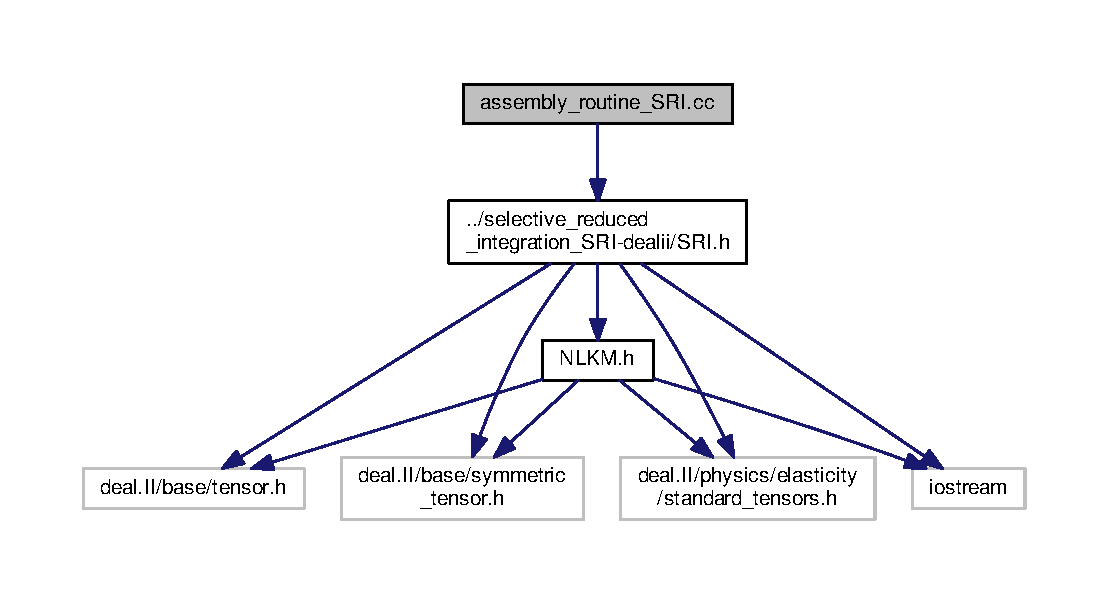
\includegraphics[width=350pt]{assembly__routine__SRI_8cc__incl}
\end{center}
\end{figure}
\subsection*{Classes}
\begin{DoxyCompactItemize}
\item 
class \hyperlink{classSolid}{Solid$<$ dim $>$}
\end{DoxyCompactItemize}
\subsection*{Functions}
\begin{DoxyCompactItemize}
\item 
{\footnotesize template$<$int dim$>$ }\\class \hyperlink{classSolid}{Solid} \hyperlink{assembly__routine__SRI_8cc_a031582e4b219de9cc57c78ebd20a2fc3}{Solid} (...)
\end{DoxyCompactItemize}
\subsection*{Variables}
\begin{DoxyCompactItemize}
\item 
const F\+E\+Values\+Extractors\+::\+Vector \hyperlink{assembly__routine__SRI_8cc_ae50a49c136e49c33fcd5a555a00009dd}{u\+\_\+fe}
\item 
const Q\+Gauss$<$ dim $>$ \hyperlink{assembly__routine__SRI_8cc_aaaceb34a5b42a4954b2e893607c1bdef}{qf\+\_\+cell}
\item 
const Q\+Gauss$<$ dim $>$ \hyperlink{assembly__routine__SRI_8cc_ab9727a7376e2656d3cd40c65ac7efb81}{qf\+\_\+cell\+\_\+\+RI}
\item 
const unsigned int \hyperlink{assembly__routine__SRI_8cc_afd52b693751274175b93a58458201e6b}{n\+\_\+q\+\_\+points}
\item 
const unsigned int \hyperlink{assembly__routine__SRI_8cc_a0b72b2a33d52b7597b87df35b5b92415}{n\+\_\+q\+\_\+points\+\_\+\+RI}
\item 
const bool \hyperlink{assembly__routine__SRI_8cc_a535468030220abae9305a26e9d7f7401}{S\+R\+I\+\_\+active} = true
\item 
\hyperlink{namespaceenums_ad159a7d6539f111883db3b07c09601a8}{enums\+::enum\+\_\+\+S\+R\+I\+\_\+type} \hyperlink{assembly__routine__SRI_8cc_a163566963ded80f68a5bbc6d04ce0adf}{S\+R\+I\+\_\+type} = \hyperlink{namespaceenums_ad159a7d6539f111883db3b07c09601a8ad2c871b65148302b24a39fac6cedfd40}{enums\+::vol\+\_\+dev\+\_\+split}
\end{DoxyCompactItemize}


\subsection{Function Documentation}
\index{assembly\+\_\+routine\+\_\+\+S\+R\+I.\+cc@{assembly\+\_\+routine\+\_\+\+S\+R\+I.\+cc}!Solid@{Solid}}
\index{Solid@{Solid}!assembly\+\_\+routine\+\_\+\+S\+R\+I.\+cc@{assembly\+\_\+routine\+\_\+\+S\+R\+I.\+cc}}
\subsubsection[{\texorpdfstring{Solid(...)}{Solid(...)}}]{\setlength{\rightskip}{0pt plus 5cm}template$<$int dim$>$ class {\bf Solid} {\bf Solid} (
\begin{DoxyParamCaption}
\item[{}]{...}
\end{DoxyParamCaption}
)}\hypertarget{assembly__routine__SRI_8cc_a031582e4b219de9cc57c78ebd20a2fc3}{}\label{assembly__routine__SRI_8cc_a031582e4b219de9cc57c78ebd20a2fc3}


Definition at line 44 of file assembly\+\_\+routine\+\_\+\+S\+R\+I.\+cc.



\subsection{Variable Documentation}
\index{assembly\+\_\+routine\+\_\+\+S\+R\+I.\+cc@{assembly\+\_\+routine\+\_\+\+S\+R\+I.\+cc}!n\+\_\+q\+\_\+points@{n\+\_\+q\+\_\+points}}
\index{n\+\_\+q\+\_\+points@{n\+\_\+q\+\_\+points}!assembly\+\_\+routine\+\_\+\+S\+R\+I.\+cc@{assembly\+\_\+routine\+\_\+\+S\+R\+I.\+cc}}
\subsubsection[{\texorpdfstring{n\+\_\+q\+\_\+points}{n_q_points}}]{\setlength{\rightskip}{0pt plus 5cm}const unsigned int n\+\_\+q\+\_\+points}\hypertarget{assembly__routine__SRI_8cc_afd52b693751274175b93a58458201e6b}{}\label{assembly__routine__SRI_8cc_afd52b693751274175b93a58458201e6b}


Definition at line 15 of file assembly\+\_\+routine\+\_\+\+S\+R\+I.\+cc.

\index{assembly\+\_\+routine\+\_\+\+S\+R\+I.\+cc@{assembly\+\_\+routine\+\_\+\+S\+R\+I.\+cc}!n\+\_\+q\+\_\+points\+\_\+\+RI@{n\+\_\+q\+\_\+points\+\_\+\+RI}}
\index{n\+\_\+q\+\_\+points\+\_\+\+RI@{n\+\_\+q\+\_\+points\+\_\+\+RI}!assembly\+\_\+routine\+\_\+\+S\+R\+I.\+cc@{assembly\+\_\+routine\+\_\+\+S\+R\+I.\+cc}}
\subsubsection[{\texorpdfstring{n\+\_\+q\+\_\+points\+\_\+\+RI}{n_q_points_RI}}]{\setlength{\rightskip}{0pt plus 5cm}const unsigned int n\+\_\+q\+\_\+points\+\_\+\+RI}\hypertarget{assembly__routine__SRI_8cc_a0b72b2a33d52b7597b87df35b5b92415}{}\label{assembly__routine__SRI_8cc_a0b72b2a33d52b7597b87df35b5b92415}


Definition at line 16 of file assembly\+\_\+routine\+\_\+\+S\+R\+I.\+cc.

\index{assembly\+\_\+routine\+\_\+\+S\+R\+I.\+cc@{assembly\+\_\+routine\+\_\+\+S\+R\+I.\+cc}!qf\+\_\+cell@{qf\+\_\+cell}}
\index{qf\+\_\+cell@{qf\+\_\+cell}!assembly\+\_\+routine\+\_\+\+S\+R\+I.\+cc@{assembly\+\_\+routine\+\_\+\+S\+R\+I.\+cc}}
\subsubsection[{\texorpdfstring{qf\+\_\+cell}{qf_cell}}]{\setlength{\rightskip}{0pt plus 5cm}const Q\+Gauss$<$dim$>$ qf\+\_\+cell}\hypertarget{assembly__routine__SRI_8cc_aaaceb34a5b42a4954b2e893607c1bdef}{}\label{assembly__routine__SRI_8cc_aaaceb34a5b42a4954b2e893607c1bdef}


Definition at line 13 of file assembly\+\_\+routine\+\_\+\+S\+R\+I.\+cc.

\index{assembly\+\_\+routine\+\_\+\+S\+R\+I.\+cc@{assembly\+\_\+routine\+\_\+\+S\+R\+I.\+cc}!qf\+\_\+cell\+\_\+\+RI@{qf\+\_\+cell\+\_\+\+RI}}
\index{qf\+\_\+cell\+\_\+\+RI@{qf\+\_\+cell\+\_\+\+RI}!assembly\+\_\+routine\+\_\+\+S\+R\+I.\+cc@{assembly\+\_\+routine\+\_\+\+S\+R\+I.\+cc}}
\subsubsection[{\texorpdfstring{qf\+\_\+cell\+\_\+\+RI}{qf_cell_RI}}]{\setlength{\rightskip}{0pt plus 5cm}const Q\+Gauss$<$dim$>$ qf\+\_\+cell\+\_\+\+RI}\hypertarget{assembly__routine__SRI_8cc_ab9727a7376e2656d3cd40c65ac7efb81}{}\label{assembly__routine__SRI_8cc_ab9727a7376e2656d3cd40c65ac7efb81}


Definition at line 14 of file assembly\+\_\+routine\+\_\+\+S\+R\+I.\+cc.

\index{assembly\+\_\+routine\+\_\+\+S\+R\+I.\+cc@{assembly\+\_\+routine\+\_\+\+S\+R\+I.\+cc}!S\+R\+I\+\_\+active@{S\+R\+I\+\_\+active}}
\index{S\+R\+I\+\_\+active@{S\+R\+I\+\_\+active}!assembly\+\_\+routine\+\_\+\+S\+R\+I.\+cc@{assembly\+\_\+routine\+\_\+\+S\+R\+I.\+cc}}
\subsubsection[{\texorpdfstring{S\+R\+I\+\_\+active}{SRI_active}}]{\setlength{\rightskip}{0pt plus 5cm}const bool S\+R\+I\+\_\+active = true}\hypertarget{assembly__routine__SRI_8cc_a535468030220abae9305a26e9d7f7401}{}\label{assembly__routine__SRI_8cc_a535468030220abae9305a26e9d7f7401}


Definition at line 20 of file assembly\+\_\+routine\+\_\+\+S\+R\+I.\+cc.

\index{assembly\+\_\+routine\+\_\+\+S\+R\+I.\+cc@{assembly\+\_\+routine\+\_\+\+S\+R\+I.\+cc}!S\+R\+I\+\_\+type@{S\+R\+I\+\_\+type}}
\index{S\+R\+I\+\_\+type@{S\+R\+I\+\_\+type}!assembly\+\_\+routine\+\_\+\+S\+R\+I.\+cc@{assembly\+\_\+routine\+\_\+\+S\+R\+I.\+cc}}
\subsubsection[{\texorpdfstring{S\+R\+I\+\_\+type}{SRI_type}}]{\setlength{\rightskip}{0pt plus 5cm}{\bf enums\+::enum\+\_\+\+S\+R\+I\+\_\+type} S\+R\+I\+\_\+type = {\bf enums\+::vol\+\_\+dev\+\_\+split}}\hypertarget{assembly__routine__SRI_8cc_a163566963ded80f68a5bbc6d04ce0adf}{}\label{assembly__routine__SRI_8cc_a163566963ded80f68a5bbc6d04ce0adf}


Definition at line 25 of file assembly\+\_\+routine\+\_\+\+S\+R\+I.\+cc.

\index{assembly\+\_\+routine\+\_\+\+S\+R\+I.\+cc@{assembly\+\_\+routine\+\_\+\+S\+R\+I.\+cc}!u\+\_\+fe@{u\+\_\+fe}}
\index{u\+\_\+fe@{u\+\_\+fe}!assembly\+\_\+routine\+\_\+\+S\+R\+I.\+cc@{assembly\+\_\+routine\+\_\+\+S\+R\+I.\+cc}}
\subsubsection[{\texorpdfstring{u\+\_\+fe}{u_fe}}]{\setlength{\rightskip}{0pt plus 5cm}const F\+E\+Values\+Extractors\+::\+Vector u\+\_\+fe}\hypertarget{assembly__routine__SRI_8cc_ae50a49c136e49c33fcd5a555a00009dd}{}\label{assembly__routine__SRI_8cc_ae50a49c136e49c33fcd5a555a00009dd}


Definition at line 6 of file assembly\+\_\+routine\+\_\+\+S\+R\+I.\+cc.


\hypertarget{mainpage_8h}{}\section{mainpage.\+h File Reference}
\label{mainpage_8h}\index{mainpage.\+h@{mainpage.\+h}}

\hypertarget{NLKM_8h}{}\section{N\+L\+K\+M.\+h File Reference}
\label{NLKM_8h}\index{N\+L\+K\+M.\+h@{N\+L\+K\+M.\+h}}
{\ttfamily \#include $<$deal.\+I\+I/base/tensor.\+h$>$}\\*
{\ttfamily \#include $<$deal.\+I\+I/base/symmetric\+\_\+tensor.\+h$>$}\\*
{\ttfamily \#include $<$deal.\+I\+I/physics/elasticity/standard\+\_\+tensors.\+h$>$}\\*
{\ttfamily \#include $<$iostream$>$}\\*
Include dependency graph for N\+L\+K\+M.\+h\+:\nopagebreak
\begin{figure}[H]
\begin{center}
\leavevmode
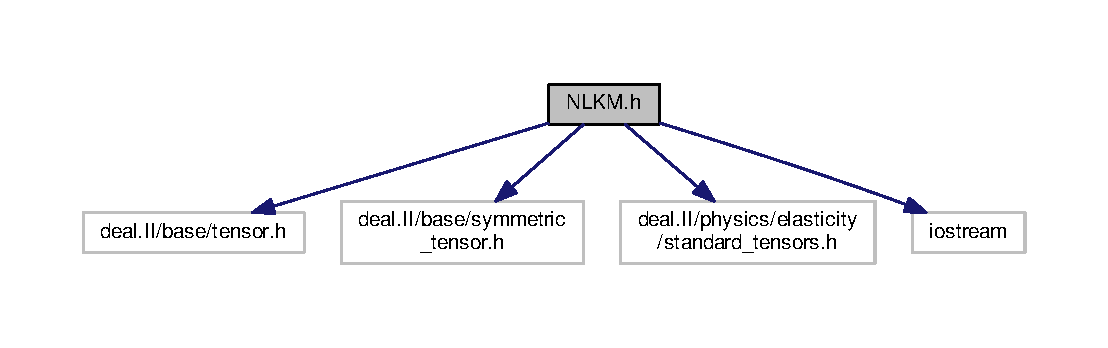
\includegraphics[width=350pt]{NLKM_8h__incl}
\end{center}
\end{figure}
This graph shows which files directly or indirectly include this file\+:\nopagebreak
\begin{figure}[H]
\begin{center}
\leavevmode
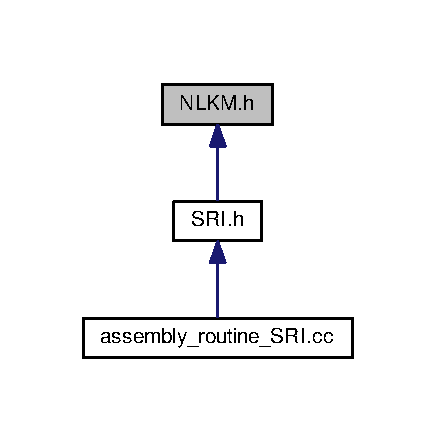
\includegraphics[width=209pt]{NLKM_8h__dep__incl}
\end{center}
\end{figure}
\subsection*{Namespaces}
\begin{DoxyCompactItemize}
\item 
 \hyperlink{namespaceNLKM}{N\+L\+KM}
\end{DoxyCompactItemize}
\subsection*{Functions}
\begin{DoxyCompactItemize}
\item 
{\footnotesize template$<$int dim$>$ }\\Symmetric\+Tensor$<$ 2, dim $>$ \hyperlink{namespaceNLKM_a1ccf48261890fc2be5d1e97f03c62ce5}{N\+L\+K\+M\+::get\+\_\+stress\+\_\+\+S\+\_\+vol} (const Tensor$<$ 2, dim $>$ \&F, const Symmetric\+Tensor$<$ 2, dim $>$ \&stress\+\_\+S)
\item 
{\footnotesize template$<$int dim$>$ }\\Symmetric\+Tensor$<$ 4, dim $>$ \hyperlink{namespaceNLKM_aa0abeda2910b5d2974905bdab35bae78}{N\+L\+K\+M\+::get\+\_\+d\+Kx\+S\+\_\+dC} (const Tensor$<$ 2, dim $>$ \&F, const Symmetric\+Tensor$<$ 2, dim $>$ \&stress\+\_\+S, const Symmetric\+Tensor$<$ 4, dim $>$ \&Tangent)
\end{DoxyCompactItemize}

\hypertarget{SRI_8h}{}\section{S\+R\+I.\+h File Reference}
\label{SRI_8h}\index{S\+R\+I.\+h@{S\+R\+I.\+h}}
{\ttfamily \#include $<$deal.\+I\+I/base/tensor.\+h$>$}\\*
{\ttfamily \#include $<$deal.\+I\+I/base/symmetric\+\_\+tensor.\+h$>$}\\*
{\ttfamily \#include $<$deal.\+I\+I/physics/elasticity/standard\+\_\+tensors.\+h$>$}\\*
{\ttfamily \#include $<$iostream$>$}\\*
{\ttfamily \#include \char`\"{}N\+L\+K\+M.\+h\char`\"{}}\\*
Include dependency graph for S\+R\+I.\+h\+:\nopagebreak
\begin{figure}[H]
\begin{center}
\leavevmode
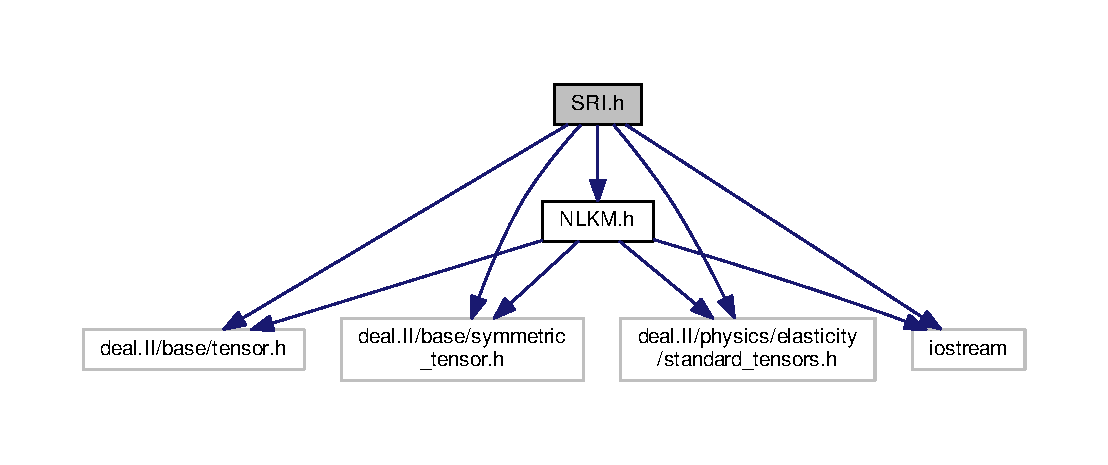
\includegraphics[width=350pt]{SRI_8h__incl}
\end{center}
\end{figure}
This graph shows which files directly or indirectly include this file\+:\nopagebreak
\begin{figure}[H]
\begin{center}
\leavevmode
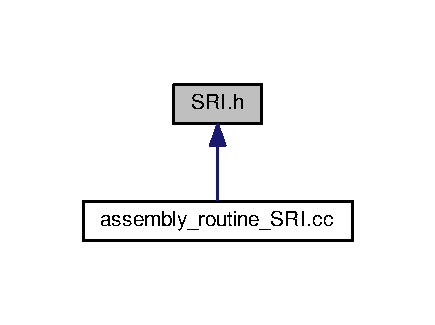
\includegraphics[width=209pt]{SRI_8h__dep__incl}
\end{center}
\end{figure}
\subsection*{Namespaces}
\begin{DoxyCompactItemize}
\item 
 \hyperlink{namespaceenums}{enums}
\item 
 \hyperlink{namespaceSRI}{S\+RI}
\end{DoxyCompactItemize}
\subsection*{Enumerations}
\begin{DoxyCompactItemize}
\item 
enum \hyperlink{namespaceenums_ad159a7d6539f111883db3b07c09601a8}{enums\+::enum\+\_\+\+S\+R\+I\+\_\+type} \{ \hyperlink{namespaceenums_ad159a7d6539f111883db3b07c09601a8ad2c871b65148302b24a39fac6cedfd40}{enums\+::vol\+\_\+dev\+\_\+split} = 0, 
\hyperlink{namespaceenums_ad159a7d6539f111883db3b07c09601a8a2754f7ec0e001029442600188c83d582}{enums\+::shear\+\_\+normal\+\_\+split} = 1
 \}
\end{DoxyCompactItemize}
\subsection*{Functions}
\begin{DoxyCompactItemize}
\item 
{\footnotesize template$<$int dim$>$ }\\void \hyperlink{namespaceSRI_add98d0fc70a6c51803dfd8c491547413}{S\+R\+I\+::prepare\+\_\+sol\+Grads} (const unsigned int \hyperlink{assembly__routine__SRI_8cc_a0b72b2a33d52b7597b87df35b5b92415}{n\+\_\+q\+\_\+points\+\_\+\+RI}, F\+E\+Values$<$ dim $>$ \&fe\+\_\+values\+\_\+ref\+\_\+\+RI, const Vector$<$ double $>$ \&current\+\_\+solution, std\+::vector$<$ Tensor$<$ 2, dim $>$ $>$ \&solution\+\_\+grads\+\_\+u)
\item 
{\footnotesize template$<$int dim$>$ }\\void \hyperlink{namespaceSRI_a369a3f624dbb7fdc2106bcc520366d24}{S\+R\+I\+::prepare\+\_\+sol2\+\_\+sol\+Grads} (const unsigned int \hyperlink{assembly__routine__SRI_8cc_a0b72b2a33d52b7597b87df35b5b92415}{n\+\_\+q\+\_\+points\+\_\+\+RI}, F\+E\+Values$<$ dim $>$ \&fe\+\_\+values\+\_\+ref\+\_\+\+RI, const Vector$<$ double $>$ \&current\+\_\+solution, std\+::vector$<$ Tensor$<$ 2, dim $>$ $>$ \&solution\+\_\+grads\+\_\+u, std\+::vector$<$ double $>$ \&phi\+\_\+n1, std\+::vector$<$ Tensor$<$ 1, dim $>$ $>$ \&solution\+\_\+grads\+\_\+phi)
\item 
bool \hyperlink{namespaceSRI_a8403675a876445cd7f069cc73aa55d05}{S\+R\+I\+::assemble\+\_\+first\+\_\+part} (const unsigned int k, const unsigned int \hyperlink{assembly__routine__SRI_8cc_afd52b693751274175b93a58458201e6b}{n\+\_\+q\+\_\+points})
\item 
Symmetric\+Tensor$<$ 2, 3 $>$ \hyperlink{namespaceSRI_aa4f8e16d0494b0945d0eadb845367ab4}{S\+R\+I\+::get\+\_\+shear\+\_\+part} (const Symmetric\+Tensor$<$ 2, 3 $>$ \&Sym\+Ten)
\item 
Symmetric\+Tensor$<$ 4, 3 $>$ \hyperlink{namespaceSRI_a41e9c32e257c2d3d3ae337cd992658ee}{S\+R\+I\+::get\+\_\+shear\+\_\+part} (const Symmetric\+Tensor$<$ 4, 3 $>$ \&Sym\+Ten)
\item 
Symmetric\+Tensor$<$ 2, 3 $>$ \hyperlink{namespaceSRI_a6fddaa4232b80942ecf98d0d5bb69d83}{S\+R\+I\+::second\+\_\+part} (const Tensor$<$ 2, 3 $>$ \&F, const Symmetric\+Tensor$<$ 2, 3 $>$ \&stress\+\_\+S, \hyperlink{namespaceenums_ad159a7d6539f111883db3b07c09601a8}{enums\+::enum\+\_\+\+S\+R\+I\+\_\+type} \hyperlink{assembly__routine__SRI_8cc_a163566963ded80f68a5bbc6d04ce0adf}{S\+R\+I\+\_\+type})
\item 
Symmetric\+Tensor$<$ 2, 3 $>$ \hyperlink{namespaceSRI_a99b236a4dfdbad69d9bc9473d1110801}{S\+R\+I\+::first\+\_\+part} (const Tensor$<$ 2, 3 $>$ \&F, const Symmetric\+Tensor$<$ 2, 3 $>$ \&stress\+\_\+S, \hyperlink{namespaceenums_ad159a7d6539f111883db3b07c09601a8}{enums\+::enum\+\_\+\+S\+R\+I\+\_\+type} \hyperlink{assembly__routine__SRI_8cc_a163566963ded80f68a5bbc6d04ce0adf}{S\+R\+I\+\_\+type})
\item 
Symmetric\+Tensor$<$ 4, 3 $>$ \hyperlink{namespaceSRI_a59dcf1c9d3d602b0d3d3044c23cb2f10}{S\+R\+I\+::second\+\_\+part} (const Tensor$<$ 2, 3 $>$ \&F, const Symmetric\+Tensor$<$ 2, 3 $>$ \&stress\+\_\+S, const Symmetric\+Tensor$<$ 4, 3 $>$ \&Tangent, \hyperlink{namespaceenums_ad159a7d6539f111883db3b07c09601a8}{enums\+::enum\+\_\+\+S\+R\+I\+\_\+type} \hyperlink{assembly__routine__SRI_8cc_a163566963ded80f68a5bbc6d04ce0adf}{S\+R\+I\+\_\+type})
\item 
Symmetric\+Tensor$<$ 4, 3 $>$ \hyperlink{namespaceSRI_a7893737600c5ccd2b127e19c13a1d516}{S\+R\+I\+::first\+\_\+part} (const Tensor$<$ 2, 3 $>$ \&F, const Symmetric\+Tensor$<$ 2, 3 $>$ \&stress\+\_\+S, const Symmetric\+Tensor$<$ 4, 3 $>$ \&Tangent, \hyperlink{namespaceenums_ad159a7d6539f111883db3b07c09601a8}{enums\+::enum\+\_\+\+S\+R\+I\+\_\+type} \hyperlink{assembly__routine__SRI_8cc_a163566963ded80f68a5bbc6d04ce0adf}{S\+R\+I\+\_\+type})
\item 
{\footnotesize template$<$int dim$>$ }\\Symmetric\+Tensor$<$ 2, dim $>$ \hyperlink{namespaceSRI_a3d489ecd63fbd10aeb4a72281196baca}{S\+R\+I\+::part} (const Tensor$<$ 2, 3 $>$ \&F, const Symmetric\+Tensor$<$ 2, 3 $>$ \&stress\+\_\+S, \hyperlink{namespaceenums_ad159a7d6539f111883db3b07c09601a8}{enums\+::enum\+\_\+\+S\+R\+I\+\_\+type} \hyperlink{assembly__routine__SRI_8cc_a163566963ded80f68a5bbc6d04ce0adf}{S\+R\+I\+\_\+type}, const unsigned int k, const unsigned int \hyperlink{assembly__routine__SRI_8cc_afd52b693751274175b93a58458201e6b}{n\+\_\+q\+\_\+points})
\item 
{\footnotesize template$<$int dim$>$ }\\Symmetric\+Tensor$<$ 4, dim $>$ \hyperlink{namespaceSRI_a206b72c5652b68159cb0211c53bc9f5c}{S\+R\+I\+::part} (const Tensor$<$ 2, 3 $>$ \&F, const Symmetric\+Tensor$<$ 2, 3 $>$ \&stress\+\_\+S, const Symmetric\+Tensor$<$ 4, 3 $>$ \&Tangent, \hyperlink{namespaceenums_ad159a7d6539f111883db3b07c09601a8}{enums\+::enum\+\_\+\+S\+R\+I\+\_\+type} \hyperlink{assembly__routine__SRI_8cc_a163566963ded80f68a5bbc6d04ce0adf}{S\+R\+I\+\_\+type}, const unsigned int k, const unsigned int \hyperlink{assembly__routine__SRI_8cc_afd52b693751274175b93a58458201e6b}{n\+\_\+q\+\_\+points})
\item 
{\footnotesize template$<$int dim$>$ }\\void \hyperlink{namespaceSRI_a304be230ce6414b79b92c2921ad38524}{S\+R\+I\+::init\+\_\+fe\+\_\+k} (F\+E\+Values$<$ dim $>$ \&fe\+\_\+values\+\_\+first\+\_\+part, F\+E\+Values$<$ dim $>$ \&fe\+\_\+values\+\_\+second\+\_\+part, const unsigned int k, const unsigned int \hyperlink{assembly__routine__SRI_8cc_afd52b693751274175b93a58458201e6b}{n\+\_\+q\+\_\+points}, F\+E\+Values$<$ dim $>$ $\ast$(\&fe\+\_\+values\+\_\+part), unsigned int \&k\+\_\+rel)
\end{DoxyCompactItemize}
\subsection*{Variables}
\begin{DoxyCompactItemize}
\item 
enum \hyperlink{namespaceenums_ad159a7d6539f111883db3b07c09601a8}{enums\+::enum\+\_\+\+S\+R\+I\+\_\+type} \hyperlink{namespaceenums_aea86a2beeb3b43f96447126c7f5dd2f3}{enums\+::\+Solid}
\end{DoxyCompactItemize}

%--- End generated contents ---

% Index
\backmatter
\newpage
\phantomsection
\clearemptydoublepage
\addcontentsline{toc}{chapter}{Index}
\printindex

\end{document}
